\documentclass[twoside]{tufte-book}

% ams
\usepackage{amssymb,amsmath}
\newcommand{\blankpage}{\newpage\hbox{}\thispagestyle{empty}\newpage}

\usepackage{ifxetex,ifluatex}
\usepackage{fixltx2e} % provides \textsubscript
\ifnum 0\ifxetex 1\fi\ifluatex 1\fi=0 % if pdftex
  \usepackage[T1]{fontenc}
  \usepackage[utf8]{inputenc}
\else % if luatex or xelatex
  \makeatletter
  \@ifpackageloaded{fontspec}{}{\usepackage{fontspec}}
  \makeatother
  \defaultfontfeatures{Ligatures=TeX,Scale=MatchLowercase}
  \makeatletter
  \@ifpackageloaded{soul}{
     \renewcommand\allcapsspacing[1]{{\addfontfeature{LetterSpace=15}#1}}
     \renewcommand\smallcapsspacing[1]{{\addfontfeature{LetterSpace=10}#1}}
   }{}
  \makeatother

\fi




% graphix
\usepackage{graphicx}
\setkeys{Gin}{width=\linewidth,totalheight=\textheight,keepaspectratio}

% booktabs
\usepackage{booktabs}

% url
\usepackage{url}

% hyperref
\usepackage{hyperref}

% units.
\usepackage{units}


\setcounter{secnumdepth}{2}

% citations


% pandoc syntax highlighting
\usepackage{color}
\usepackage{fancyvrb}
\newcommand{\VerbBar}{|}
\newcommand{\VERB}{\Verb[commandchars=\\\{\}]}
\DefineVerbatimEnvironment{Highlighting}{Verbatim}{commandchars=\\\{\}}
% Add ',fontsize=\small' for more characters per line
\newenvironment{Shaded}{}{}
\newcommand{\AlertTok}[1]{\textcolor[rgb]{1.00,0.00,0.00}{\textbf{#1}}}
\newcommand{\AnnotationTok}[1]{\textcolor[rgb]{0.38,0.63,0.69}{\textbf{\textit{#1}}}}
\newcommand{\AttributeTok}[1]{\textcolor[rgb]{0.49,0.56,0.16}{#1}}
\newcommand{\BaseNTok}[1]{\textcolor[rgb]{0.25,0.63,0.44}{#1}}
\newcommand{\BuiltInTok}[1]{\textcolor[rgb]{0.00,0.50,0.00}{#1}}
\newcommand{\CharTok}[1]{\textcolor[rgb]{0.25,0.44,0.63}{#1}}
\newcommand{\CommentTok}[1]{\textcolor[rgb]{0.38,0.63,0.69}{\textit{#1}}}
\newcommand{\CommentVarTok}[1]{\textcolor[rgb]{0.38,0.63,0.69}{\textbf{\textit{#1}}}}
\newcommand{\ConstantTok}[1]{\textcolor[rgb]{0.53,0.00,0.00}{#1}}
\newcommand{\ControlFlowTok}[1]{\textcolor[rgb]{0.00,0.44,0.13}{\textbf{#1}}}
\newcommand{\DataTypeTok}[1]{\textcolor[rgb]{0.56,0.13,0.00}{#1}}
\newcommand{\DecValTok}[1]{\textcolor[rgb]{0.25,0.63,0.44}{#1}}
\newcommand{\DocumentationTok}[1]{\textcolor[rgb]{0.73,0.13,0.13}{\textit{#1}}}
\newcommand{\ErrorTok}[1]{\textcolor[rgb]{1.00,0.00,0.00}{\textbf{#1}}}
\newcommand{\ExtensionTok}[1]{#1}
\newcommand{\FloatTok}[1]{\textcolor[rgb]{0.25,0.63,0.44}{#1}}
\newcommand{\FunctionTok}[1]{\textcolor[rgb]{0.02,0.16,0.49}{#1}}
\newcommand{\ImportTok}[1]{\textcolor[rgb]{0.00,0.50,0.00}{\textbf{#1}}}
\newcommand{\InformationTok}[1]{\textcolor[rgb]{0.38,0.63,0.69}{\textbf{\textit{#1}}}}
\newcommand{\KeywordTok}[1]{\textcolor[rgb]{0.00,0.44,0.13}{\textbf{#1}}}
\newcommand{\NormalTok}[1]{#1}
\newcommand{\OperatorTok}[1]{\textcolor[rgb]{0.40,0.40,0.40}{#1}}
\newcommand{\OtherTok}[1]{\textcolor[rgb]{0.00,0.44,0.13}{#1}}
\newcommand{\PreprocessorTok}[1]{\textcolor[rgb]{0.74,0.48,0.00}{#1}}
\newcommand{\RegionMarkerTok}[1]{#1}
\newcommand{\SpecialCharTok}[1]{\textcolor[rgb]{0.25,0.44,0.63}{#1}}
\newcommand{\SpecialStringTok}[1]{\textcolor[rgb]{0.73,0.40,0.53}{#1}}
\newcommand{\StringTok}[1]{\textcolor[rgb]{0.25,0.44,0.63}{#1}}
\newcommand{\VariableTok}[1]{\textcolor[rgb]{0.10,0.09,0.49}{#1}}
\newcommand{\VerbatimStringTok}[1]{\textcolor[rgb]{0.25,0.44,0.63}{#1}}
\newcommand{\WarningTok}[1]{\textcolor[rgb]{0.38,0.63,0.69}{\textbf{\textit{#1}}}}

% table with pandoc
\usepackage{longtable,booktabs,array}
\usepackage{calc} % for calculating minipage widths
% Correct order of tables after \paragraph or \subparagraph
\usepackage{etoolbox}
\makeatletter
\patchcmd\longtable{\par}{\if@noskipsec\mbox{}\fi\par}{}{}
\makeatother
% Allow footnotes in longtable head/foot
\IfFileExists{footnotehyper.sty}{\usepackage{footnotehyper}}{\usepackage{footnote}}
\makesavenoteenv{longtable}

% multiplecol
\usepackage{multicol}

% strikeout
\usepackage[normalem]{ulem}

% morefloats
\usepackage{morefloats}


% tightlist macro required by pandoc >= 1.14
\providecommand{\tightlist}{%
  \setlength{\itemsep}{0pt}\setlength{\parskip}{0pt}}

% title / author / date
\title{Creating Exercises and Exams With the R Package rqti}
\author{Johannes Titz and Andrey Shevandrin}
\date{2024-09-06}

\usepackage{fvextra}
\DefineVerbatimEnvironment{Highlighting}{Verbatim}{
  showspaces = false,
  showtabs = false,
  frame = leftline,
  vspace = 5pt,
  commandchars=\\\{\}
}

\usepackage{svg}
\usepackage{fvextra}
\usepackage{booktabs}
\usepackage{longtable}
\usepackage{array}
\usepackage{multirow}
\usepackage{wrapfig}
\usepackage{float}
\usepackage{colortbl}
\usepackage{pdflscape}
\usepackage{tabu}
\usepackage{threeparttable}
\usepackage{threeparttablex}
\usepackage[normalem]{ulem}
\usepackage{makecell}
\usepackage{xcolor}


\makeatletter

\fancypagestyle{mystyle}{%
\fancyhf{}%
\renewcommand{\chaptermark}[1]{\markboth{##1}{}}%
\fancyhead[LE]{\thepage\quad\smallcaps{\newlinetospace{\leftmark}}}%
\fancyhead[RO]{\smallcaps{\newlinetospace{\@author}}\quad\thepage}%
}
\makeatother


\begin{document}

\maketitle


\fancyhead{}
{
\setcounter{tocdepth}{1}
\tableofcontents
}

\chapter*{Foreword}\label{foreword}

This book is a printed version of our online documentation for the \texttt{rqti} package, available at \url{https://shevandrin.github.io/rqti/}, with a few minor modifications. Please note that this book has not been copy-edited and should not be considered a finished product. But then again, what is truly finished these days? Think of this document as a perpetual beta, evolving alongside the package.

You may come across minor issues like spelling errors, awkward phrasing, or poor typesetting. More significant problems could also arise, such as code listings that no longer run correctly or figures that fail to display the correct content. Additionally, some important topics, such as how to import QTI data for analysis, are not yet covered. We are committed to addressing these issues and enhancing this documentation over time. However, we believe that this resource already offers substantial value to anyone using our package, which is why we are providing this print version.

Note that this material is licensed under CC BY SA \copyright\ Johannes Titz and Andrey Shevandrin, 2024.

We express our deepest gratitude to the \emph{Stiftung für Innovation in der Hochschullehre}, whose financial support from 2022 to 2024 made the development of the \texttt{rqti} package possible.\footnote{project MEME, see \url{https://stiftung-hochschullehre.de/projekt/meme/}} Without their backing, the \texttt{rqti} package would not have come to life. Now that it has, we not only eagerly recommend it to our colleagues but also frequently use it ourselves---and often find ourselves revisiting this documentation. We hope you will find it as valuable as we do.

\vspace{0.5cm}

\noindent Johannes Titz and Andrey Shevandrin\\
Chemnitz, September 2024

\pagestyle{mystyle}
\chapter{Introduction to rqti}\label{introduction-to-rqti}

The \texttt{rqti} package is designed to be a powerful, stand-alone R library for creating exercises, exams, and questionnaires that fully comply with the \href{https://www.imsglobal.org/question/qtiv2p1/imsqti_implv2p1.html}{QTI v2.1 standard}. This tool empowers users to generate QTI-compliant content directly from R, offering the flexibility to render tasks locally (using qtijs) or seamlessly integrate them into learning management systems like OPAL.

Our primary target audience includes instructors specializing in research methods and statistics who want to leverage R's capabilities while adhering to the QTI standard. In particular, those utilizing OPAL will find \texttt{rqti} especially beneficial, as it fully leverages OPAL's robust API for smooth integration. However, the package is also suitable for other learning management systems that support the QTI standard.

The versatility of QTI goes beyond exercises and exams; it also supports the creation of comprehensive questionnaires, making \texttt{rqti} an invaluable tool for a wide range of educational and research applications.

\section{Installation}\label{installation}

The \texttt{rqti} package is available on CRAN, ensuring easy installation and access to its features:

\begin{Shaded}
\begin{Highlighting}[]
\FunctionTok{install.packages}\NormalTok{(}\StringTok{"rqti"}\NormalTok{)}
\end{Highlighting}
\end{Shaded}

\section{Quick start}\label{quick-start}

In RStudio, start by navigating to \emph{File} \textrightarrow{} \emph{New Project}, and then select \textbf{rqti Project} as the project type. For a quick start, you can proceed with the default settings. If you prefer to customize the options, make sure to select \emph{YES} for \emph{Create Templates}---this will generate RMarkdown templates tailored for different task types.

Once your project is created, open one of the templates from the working directory (e.g., \texttt{gap/gap.Rmd}). To preview it, simply click \emph{Knit}. The output will be displayed in the RStudio Viewer or in a new browser window if you are working outside of RStudio.

Explore the other templates to familiarize yourself with the various features and task types that \texttt{rqti} supports. This will help you create tasks that align with your specific needs.

To learn how to create sections and tests, start by reviewing the \emph{main.R} file in your working directory. This file provides a foundational understanding of structuring your work. For more detailed information, you can refer to Chapter \ref{sections-and-tests} \href{Chapters/section.html}{Sections and Tests}.

To add more templates, create a new RMarkdown file. In RStudio, go to \emph{File} \textrightarrow{} \emph{New File} \textrightarrow{} \emph{R Markdown} \textrightarrow{} \emph{From Template}, and choose one that ends with \{rqti\}. The simpler templates focus on basic parameters, while the more advanced templates showcase additional settings and customization options. After selecting a template, click the \emph{Knit} button to render the task in the viewer pane.

While the templates are generally intuitive, you can refer to other Chapters of the documentation for detailed guidance on specific task types. This will help you fully utilize the features of \texttt{rqti} for your projects. The following task types are available and explained in the corresponding chapters:

\begin{itemize}
\tightlist
\item
  \ref{single-choice-tasks} \href{Chapters/singlechoice.html}{Single-Choice tasks}
\item
  \ref{multiple-choice-tasks} \href{Chapters/multiplechoice.html}{Multiple-Choice tasks}
\item
  \ref{essay-tasks} \href{Chapters/essay.html}{Essay tasks}
\item
  \ref{gap-tasks} \href{Chapters/gap.html}{Gap tasks}
\item
  \ref{dropdown-tasks} \href{Chapters/dropdown.html}{Dropdown tasks}
\item
  \ref{order-tasks} \href{Chapters/order.html}{Order tasks}
\item
  \ref{directed-pair-tasks} \href{Chapters/directedpairs.html}{Directed Pair tasks}
\item
  \ref{table-tasks} \href{Chapters/table.html}{Table tasks}
\end{itemize}

To add metadata to your tasks, refer to Chapter \ref{adding-metadata} \href{Chapters/adding_metadata.html}{Adding metadata}.
To integrate various tasks into a test, refer to Chapter \ref{sections-and-tests} \href{Chapters/section.html}{Sections and Tests}.
For users of the learning management system OPAL, explore Chapter \ref{working-with-the-opal-api} \href{Chapters/api_opal.html}{Working with the OPAL API}.

\section{General workflow}\label{general-workflow}

The fundamental workflow with the \texttt{rqti} package involves the following steps:

\begin{enumerate}
\def\labelenumi{\arabic{enumi}.}
\tightlist
\item
  Create task files.

  \begin{itemize}
  \tightlist
  \item
    Start by generating an Rmd document. You can either start from scratch or leverage Rmd templates ending with the suffix~\texttt{\{rqti\}}.
  \item
    Create a section titled \texttt{\#\ question} and construct your interactions (gaps, choices, etc.) Utilize \texttt{rqti} helper functions where applicable.
  \item
    Specify additional attributes in the YAML section. Detailed explanations for all types are available in the following sections of this manual.
  \item
    Choose a previewer: Either qtijs (\texttt{knit:\ rqti::render\_qtijs}), for local rendering, or the learning management system Opal (\texttt{knit:\ rqti::render\_opal}). Note that Opal usage requires prior setup, which is explained in Chapter \ref{working-with-the-opal-api} \href{Chapters/api_opal.html}{Working with the Opal API}.
  \item
    Verify if your task appears as desired. Make adjustments until you are satisfied.
  \end{itemize}
\item
  Create sections and tests based on your task files.
\item
  Write the test (xml) to disk according to the QTI standard and upload the test file to your learning management system.
\item
  Download results data from your learning management system and import them with the \texttt{rqti} package for statistical analysis.
\end{enumerate}

Each step involves specific \texttt{rqti} functions, with the most useful ones illustrated in Figure \ref{workflow}

\begin{figure*}
\centering
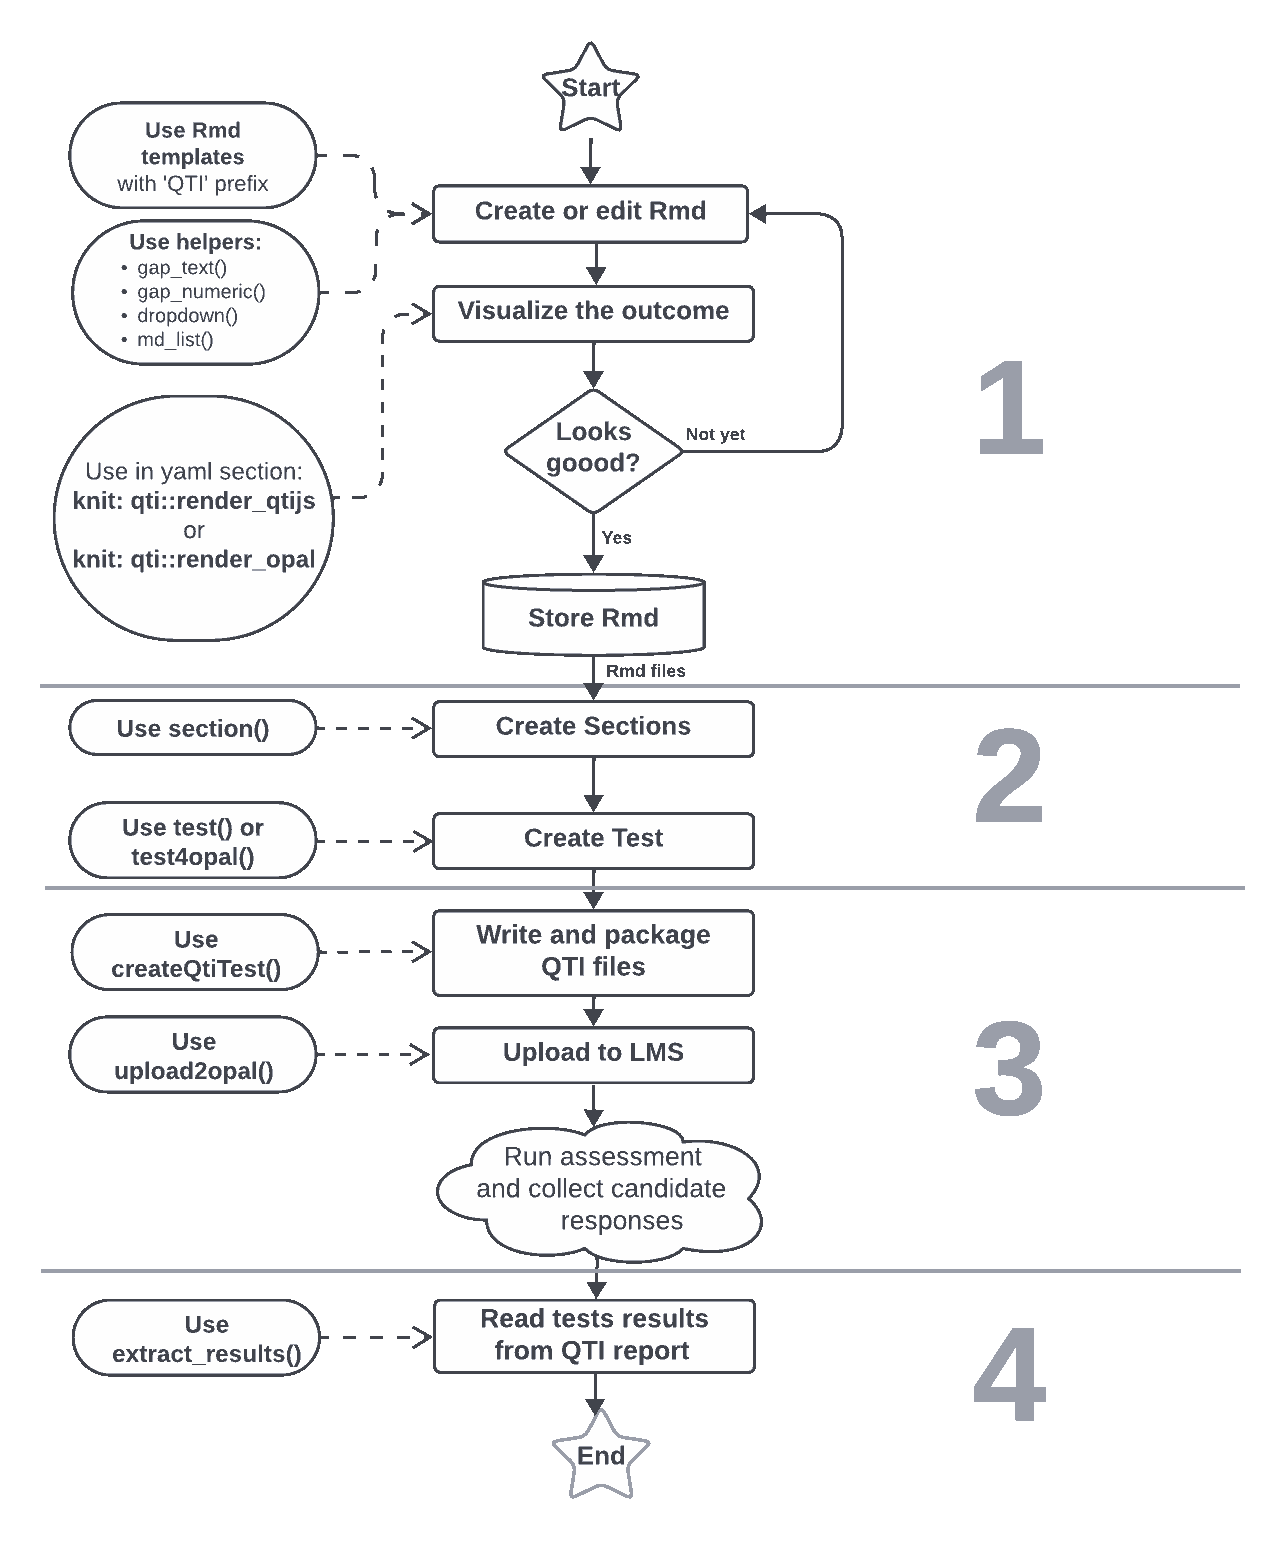
\includegraphics[width=1\textwidth,height=\textheight]{images/workflow.png}
\caption{\label{workflow}Basic workflow to create tasks and tests with rqti}
\end{figure*}

The most effective way to grasp the workflow is to create a simple task, such as \emph{Single-Choice} as demonstrated in Chapter \ref{single-choice-tasks} \href{Chapters/singlechoice.html}{Single-Choice tasks}. Once you have completed that, explore the other task types discussed in the subsequent chapters.

\section{Support and Bug Reports}\label{support-and-bug-reports}

Should you find any missing features or encounter issues, please do not hesitate to inform us via email (\href{mailto:shevandrin@gmail.com}{\nolinkurl{shevandrin@gmail.com}}) or open an issue on GitHub (\url{https://github.com/shevandrin/rqti/issues}). We will offer support until the project's funding concludes in September 2024. Following that, we will maintain a stable, usable version, with support for new features provided as time permits.

\chapter{Single-Choice tasks}\label{single-choice-tasks}

Please note that this is the first type of task described in this manual, and as such, it may be more detailed than those that follow. Our goal is to emphasize key points that might not be as thoroughly covered in later Chapters. For this reason, we recommend reading through this Chapter carefully before diving into the task types that most interest you.

\section{Minimum version}\label{minimum-version}

The simplest task type in the \texttt{rqti} package is single choice. A template is automatically created when you initiate an \texttt{rqti} project through RStudio. Alternatively, it can be added by clicking on \texttt{New\ file\ \textrightarrow{}\ R\ Markdown\ \textrightarrow{}\ From\ Template}. The \texttt{rqti} templates end with \texttt{\{rqti\}}. Here we look at the templates \texttt{singlechoice\ (simple)} and \texttt{singlechoice\ (complex)}.

The minimum you need to provide is the \texttt{type:\ sc} (or the equivalent \texttt{type:\ singlechoice}, or \texttt{type:\ schoice}) in the YAML-section and a list with at least two elements in a section called \textbf{\# question}:

\begin{Shaded}
\begin{Highlighting}
---
type: sc
knit: rqti::render_qtijs
---

# question

An alpha error of 5% means that:

- There is a 5% probability that you will mistakenly reject the null hypothesis,
when it is actually correct. <!-- First option is treated as the correct one by
default. -->
- There is a 5% probability that the null hypothesis is correct.
- There is a 5% probability that you will mistakenly reject the alternative
hypothesis, when it is correct.
- The test power is 95%.

# feedback

The correct interpretation is:

There is a 5% probability that you will mistakenly reject the null hypothesis,
when it is correct.

This is based on the typical understanding of a 5% significance level in
hypothesis testing, which means that you are willing to accept a 5% chance of
making a Type I error.
\end{Highlighting}
\end{Shaded}

Note that in this example, a feedback section was also provided. This is optional, but usually it is a good idea to give some explanation for students.

Additionally, note that the \texttt{knit} parameter is set to a custom \texttt{rqti} function, which streamlines the preview process. While this is optional, it significantly simplifies the workflow. Without it, the default preview will be a basic HTML file. By including our custom knit function, you will get a more realistic preview that allows for interaction with the task.

To preview the final result, simply click the \emph{Knit} button in RStudio (if you are not using RStudio, call \texttt{render\_qtijs} on the file). This will generate a QTI XML file and render it in the viewer pane using QTIJS. If you are not using RStudio, you can also open the server URL displayed in the console directly in your browser for the same preview experience.

You can now interact with the task by selecting an option and then clicking \texttt{Submit} in the top right corner. By default, after submitting, the feedback and reached points are displayed as shown in Figure \ref{sc1qtijs}.

\begin{figure*}
\centering
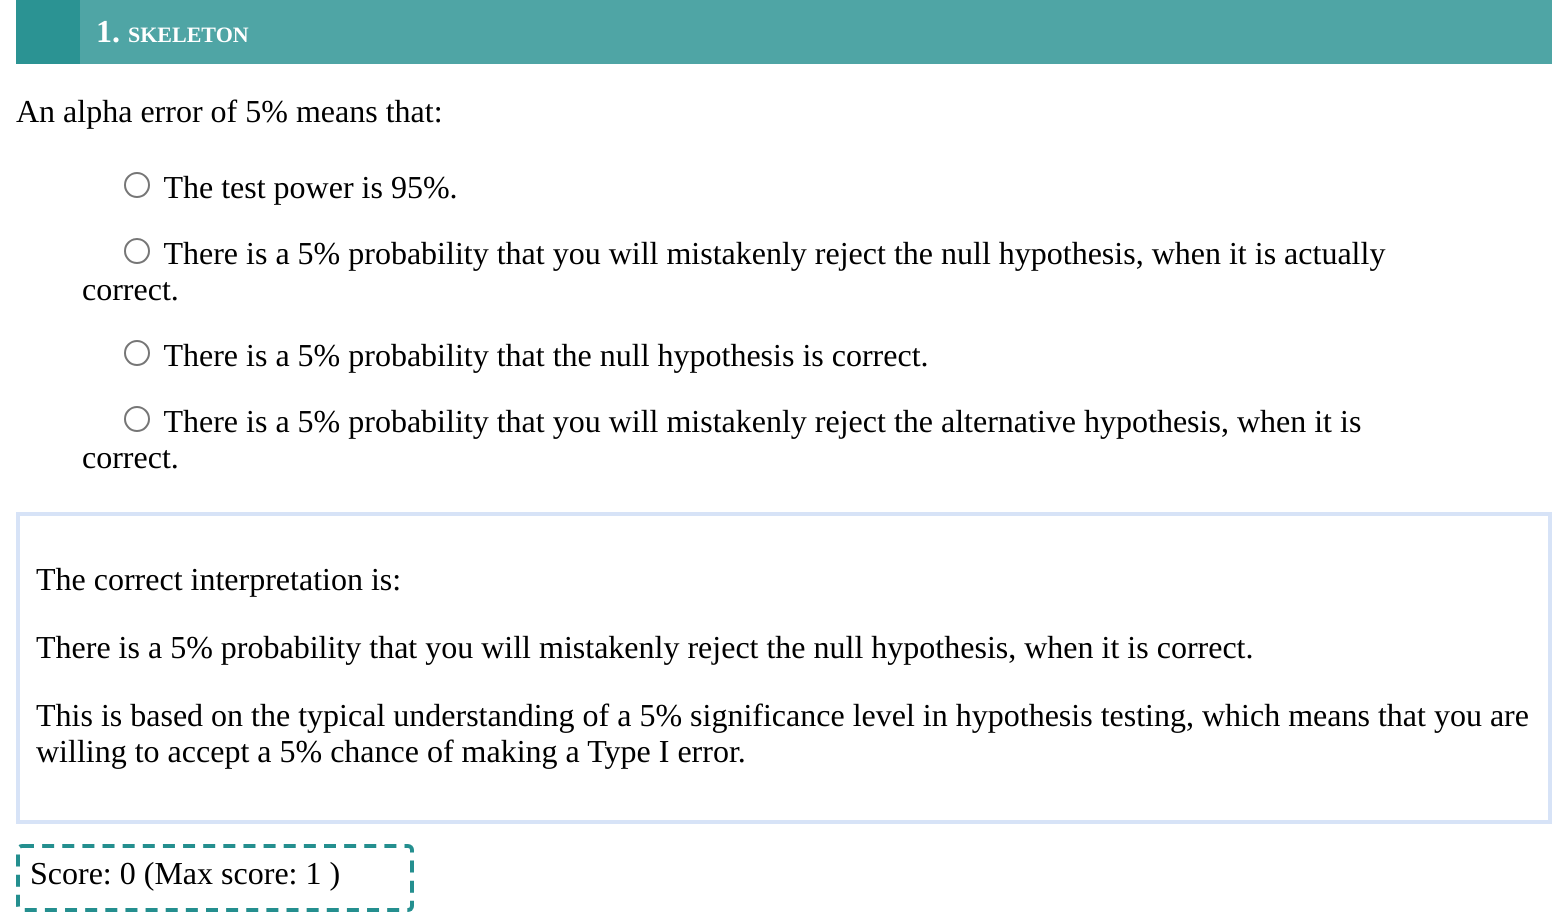
\includegraphics[width=1\textwidth,height=\textheight]{images/xml/scfb.jpg}
\caption{\label{sc1qtijs}Preview of single choice task with feedback rendered by QTIJS}
\end{figure*}

The corresponding xml file is created in the same folder as the Rmd file if you click the Knit-Button.

Many learning management systems can directly import a QTI-XML-file, so all you need to do is upload the generated file. Compositions of tasks are covered in Chapter \ref{sections-and-tests} \href{section.html}{Sections and Tests}.

If you happen to use OPAL/ONYX, you can also upload your tasks directly by modifying the knit parameter:

\begin{Shaded}
\begin{Highlighting}[]
\NormalTok{knit}\SpecialCharTok{:}\NormalTok{ rqti}\SpecialCharTok{::}\NormalTok{render\_opal}
\end{Highlighting}
\end{Shaded}

This will upload the file and open a browser with the OPAL url. It should look like in Figure \ref{sc1opal}.

\begin{figure}
\centering
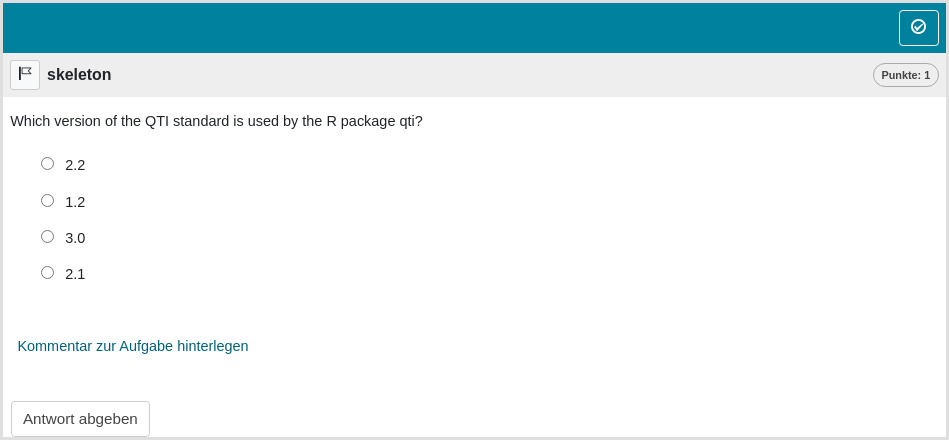
\includegraphics[width=1\textwidth,height=\textheight]{images/singlechoice-simple.jpg}
\caption{\label{sc1opal}Single choice task rendered in OPAL}
\end{figure}

Setting up OPAL requires some additional steps, which are covered in Chapter \ref{working-with-the-opal-api} \href{api_opal.html}{Working with the OPAL API}.

By default the rights of the uploaded material in OPAL are set to public, so no authentication is required to view the material. Otherwise you have to login into OPAL, which will log you out in the API. Please take this into account when testing your material. Without changing the defaults anyone with the link has access to your task.

\section{Syntax explained}\label{syntax-explained}

Let us have a closer look at the input file.

\begin{Shaded}
\begin{Highlighting}
---
type: sc
knit: rqti::render_qtijs
---

# question

An alpha error of 5% means that:

- There is a 5% probability that you will mistakenly reject the null hypothesis,
when it is actually correct. <!-- First option is treated as the correct one by
default. -->
- There is a 5% probability that the null hypothesis is correct.
- There is a 5% probability that you will mistakenly reject the alternative
hypothesis, when it is correct.
- The test power is 95%.

# feedback

The correct interpretation is:

There is a 5% probability that you will mistakenly reject the null hypothesis,
when it is correct.

This is based on the typical understanding of a 5% significance level in
hypothesis testing, which means that you are willing to accept a 5% chance of
making a Type I error.
\end{Highlighting}
\end{Shaded}

Note that you do not necessarily need to specify which list element is correct. The first one is treated as the correct one, which is a useful shortcut. If you communicate this to your collaborators, it is also much easier to read. They do not need to look anywhere else in the file for checking the correct answer.

Of course you can specify the correct choice if need be. Our preferred way of doing this is by putting asterisks around this option. For instance:

\begin{Shaded}
\begin{Highlighting}[]
\AnnotationTok{Choose the correct one:}

\SpecialStringTok{{-} }\NormalTok{A}
\SpecialStringTok{{-} }\NormalTok{B}
\SpecialStringTok{{-} }\NormalTok{*C* }\CommentTok{\textless{}!{-}{-} treated as correct {-}{-}\textgreater{}}
\SpecialStringTok{{-} }\NormalTok{D}
\end{Highlighting}
\end{Shaded}

Once again, this is much easier to read than providing the solution somewhere else (e.g.~in the YAML section). Furthermore, producing a preview as html directly shows you which element is correct. If you want to use italics in your choice, you can also wrap the correct solution in emphasize tags: \texttt{\textless{}em\textgreater{}a\ choice\ with\ *some\ italics*\textless{}/em\textgreater{}}.

An important note: Do not forget to put a blank line before your question and the answer list, otherwise the list will not be a proper list:

\begin{Shaded}
\begin{Highlighting}[]
\NormalTok{A question text that is not separated by a blank line}
\NormalTok{{-} A}
\NormalTok{{-} B}
\NormalTok{{-} C}
\NormalTok{{-} D}
\end{Highlighting}
\end{Shaded}

Renders as:

\begin{quote}
A question text that is not separated by a blank line - A - B - C - D
\end{quote}

\section{More control}\label{more-control}

If you want to have more fine-grained control, consider the RMD template \texttt{singlechoice-complex}, which uses more YAML attributes. In addition you can also set feedback for correct and incorrect responses.

\begin{Shaded}
\begin{Highlighting}
---
type: sc # equivalent to singlechoice and schoice
knit: rqti::render_qtijs # if you do not want our preview renderer, remove this
identifier: sc001 # think twice about this id for later data analysis!
title: A meaningful title that can be displayed in the LMS
shuffle: false # random order of choices
orientation: horizontal # OR horizontal
points: 0.5
calculator: scientific # OPAL specific attribute
files: attachment.pdf # OPAL scpecific attribute
---

# question

Which version of the QTI standard is used by the R package rqti?

- 1.2
- *2.1* <!--Mark correct solution with asterisks-->
- 2.2
- 3.0

# feedback+

Nice. (Only displayed when the solution is correct.)

# feedback-

Try again. (Only displayed if the solution is not correct.)

<!-- If you prefer general feedback, just use the the section # feedback and
delete the other feedback sections-->
\end{Highlighting}
\end{Shaded}

Which renders in OPAL as shown in Figure \ref{sc2opal}.

\begin{figure*}
\centering
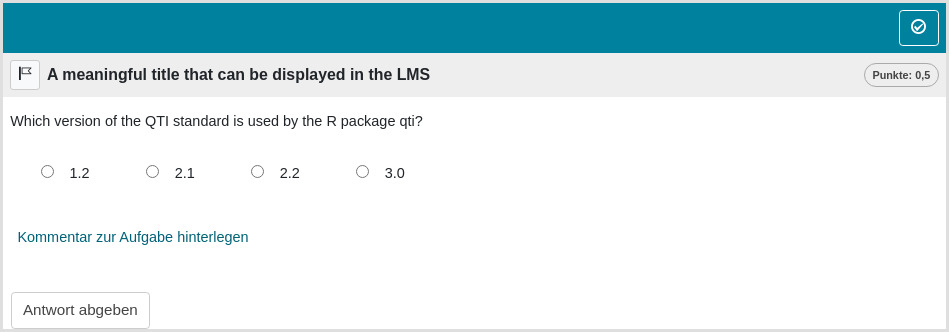
\includegraphics[width=1\textwidth,height=\textheight]{images/singlechoice-complex.jpg}
\caption{\label{sc2opal}More complex single choice task rendered in OPAL}
\end{figure*}
\newpage
Notably, the choices are now displayed horizontally, and the title and points have been updated. The next section provides a detailed explanation of all YAML attributes.

\section{YAML attributes}\label{YAML-attributes}

\noindent\textbf{type}\label{type}

Has to be \texttt{singlechoice} or \texttt{sc} (a shortcut for singlechoice) or \texttt{schoice} (compatible with \texttt{exams} package)

\noindent\textbf{identifier}\label{identifier}

This is the ID of the task, useful for later data analysis of results. The default is the file name. If you are doing extensive data analysis later on, it makes sense to specify a meaningful identifier. In all other cases, the file name should be fine.

\noindent\textbf{title}\label{title}

Title of the task. Can be displayed to students depending on the learning management system settings. Default is the file name.

\noindent\textbf{shuffle}\label{shuffle}

If \texttt{true} (the default), randomizes the order of the choices. Only in rare occasions it makes sense to have a strict order of choices (setting shuffle to \texttt{false}).

\noindent\textbf{orientation}\label{orientation}

Should the items be displayed in \texttt{vertical} or \texttt{horizontal} mode? Default is \texttt{vertical}.

\noindent\textbf{points}\label{points}

How many points are given for the correct solution. Default is 1.

\noindent\textbf{calculator}\label{calculator}

If a calculator is required for this task, you need to assign the `calculator' attribute the type `simple' or `scientific'. This only works on OPAL.

\noindent\textbf{files}\label{files}

If additional files are required to complete this task, you need to assign the `files' attribute a single file path or a list of paths to these files. Keep these additional files in the same folder with Rmd. This only works on OPAL.

\section{Feedback}\label{feedback}

Feedback can be provided with the section

\begin{itemize}
\tightlist
\item
  \textbf{\# feedback} (general feedback, displayed every time, without conditions)
\item
  \textbf{\# feedback+} (only provided if student reaches all points)
\item
  \textbf{\# feedback-} (only provided if student does not reach all points)
\end{itemize}

We typically prefer providing comprehensive feedback rather than conditional feedback. Basically, we never use feedback+ and feedback-. It is often more effective to present the entire solution, organized into manageable chunks that users can expand or collapse, such as HTML elements with \texttt{\textless{}details\textgreater{}} and \texttt{\textless{}summary\textgreater{}} tags. To give an example:

\begin{Shaded}
\begin{Highlighting}[]
\DataTypeTok{\textless{}}\KeywordTok{details}\DataTypeTok{\textgreater{}\textless{}}\KeywordTok{summary}\DataTypeTok{\textgreater{}}\NormalTok{Question1}\DataTypeTok{\textless{}/}\KeywordTok{summary}\DataTypeTok{\textgreater{}}
\NormalTok{  Provide Feedback for Question 1}
\DataTypeTok{\textless{}/}\KeywordTok{details}\DataTypeTok{\textgreater{}}
\DataTypeTok{\textless{}}\KeywordTok{details}\DataTypeTok{\textgreater{}\textless{}}\KeywordTok{summary}\DataTypeTok{\textgreater{}}\NormalTok{Question 2}\DataTypeTok{\textless{}/}\KeywordTok{summary}\DataTypeTok{\textgreater{}}
\NormalTok{  Provide Feedback for Question 2}
\DataTypeTok{\textless{}/}\KeywordTok{details}\DataTypeTok{\textgreater{}}
\end{Highlighting}
\end{Shaded}

will render as:

\noindent\textrightarrow{} Question 1\\
\noindent\textrightarrow{} Question 2\\

By clicking on the arrows, the details will unfold. Thus, there is no need to go beyond using the general feedback.

\section{List of answers as a variable}\label{list-of-answers-as-a-variable}

For more complex tasks the list of answers is often just available as a variable. In this case you can use the helper function \texttt{mdlist} to convert the vector into a markdown list:

\begin{Shaded}
\begin{Highlighting}[]
\FunctionTok{mdlist}\NormalTok{(}\FunctionTok{c}\NormalTok{(}\FloatTok{1.2}\NormalTok{, }\FloatTok{2.1}\NormalTok{, }\FloatTok{2.2}\NormalTok{, }\FloatTok{3.0}\NormalTok{), }\AttributeTok{solutions =} \DecValTok{2}\NormalTok{)}
\NormalTok{[}\DecValTok{1}\NormalTok{] }\StringTok{"{-} 1.2}\SpecialCharTok{\textbackslash{}n}\StringTok{{-} *2.1*}\SpecialCharTok{\textbackslash{}n}\StringTok{{-} 2.2}\SpecialCharTok{\textbackslash{}n}\StringTok{{-} 3"}
\end{Highlighting}
\end{Shaded}

\section{Some advice on single choice tasks}\label{some-advice-on-single-choice-tasks}

From a psychometric standpoint, single-choice tasks are often the least effective option for assessing ability. This is primarily because guessing cannot be entirely ruled out, leading to weaker psychometric properties compared to similar content presented in gap tasks.

For example, the \texttt{exams} package, an alternative R package for test creation, frequently converts numeric gaps into single-choice tasks. However, we believe this approach is justified only when the learning management system either does not support gap tasks, provides inadequate support, or the instructor requires printed exams with automated grading. In all other cases, using numeric or string gaps is generally more effective.

In some cases, single-choice tasks may be unavoidable. For instance, when determining whether a statistical test is significant, there are only two possible answers. In such situations, we suggest asking multiple related questions rather than relying on a single one. Additionally, assigning fewer points to single-choice tasks can help mitigate the effects of guessing.

If you have multiple single-choice tasks with identical answer options, consider using a match table instead (see Chapter \ref{table-tasks} \href{table.html}{Table tasks}).

In conclusion, it is advisable to avoid single-choice tasks whenever possible. Specifically, refrain from converting numeric gap tasks into single-choice format unless absolutely necessary. If single-choice tasks are unavoidable, consider asking multiple related questions or using a match table. Additionally, reducing the weight of single-choice tasks in the overall grading can help create a more balanced and fair assessment.

\chapter{Multiple-Choice tasks}\label{multiple-choice-tasks}

This is just a normal multiple choice task.

\section{Minimum version}\label{minimum-version-1}

A minimum template is automatically created when you initiate an \texttt{rqti} project through RStudio. Alternatively, it can be added by clicking on \texttt{New\ file\ \textrightarrow{}\ R\ Markdown\ \textrightarrow{}\ From\ Template}. The \texttt{rqti} templates end with \texttt{\{rqti\}}. Here we look at the templates \texttt{multiplechoice\ (simple)} and \texttt{multiplechoice\ (complex)}.

The minimum you need to provide is the \texttt{type:\ mpc} (or the equivalent \texttt{type:\ multiplechoice} or \texttt{type:\ mchoice}) in the YAML-section and a list with at least two elements in a section called \textbf{\# question}:

\begin{Shaded}
\begin{Highlighting}
---
type: mpc
knit: rqti::render_qtijs
---

# question

Which exercise types are supported by the R package rqti?

- *dropdown list*
- *gaps*
- programming language evaluation
- drawing

# feedback

All basic types of QTI are supported, including dropdown list. More advanced
exercises (as available in OPAL/ONYX) are not yet supported because they are LMS
specific.
\end{Highlighting}
\end{Shaded}

Note that in this example, a feedback section was also provided. This is optional, but usually it is a good idea to give some explanation for students.

Further note that the \texttt{knit} parameter is set to the custom \texttt{rqti} knit function, which will handle the preview. Clicking the Knit button in RStudio produces the output in Figure \ref{mpc1qtijs}.

\begin{figure*}
\centering
\includegraphics[width=1\textwidth,height=\textheight]{images/xml/multiplechoice-simple.jpg}
\caption{\label{mpc1qtijs}Multiple choice task rendered in qtijs}
\end{figure*}

You can also use the OPAL (set it up before, see Chapter \ref{working-with-the-opal-api} \href{api_opal.html}{Working with the OPAL API}) render function (\texttt{knit:\ rqti::render\_opal}), which should produce the output in Figure \ref{mpc1opal}.

\begin{figure}
\centering
\includegraphics[width=1\textwidth,height=\textheight]{images/multiplechoice-simple.jpg}
\caption{\label{mpc1opal}Multiple choice task rendered in OPAL}
\end{figure}

Multiple-choice tasks function similarly to single-choice tasks, with the key difference being that multiple (or no) answers can be correct. To indicate the correct options, surround them with asterisks. If you need to use italics within the choices themselves, enclose the entire question in \texttt{\textless{}em\textgreater{}\textless{}/em\textgreater{}} tags to avoid conflicts.

By default, the total points available for a question are calculated as \(0.5n\), where \(n\) is the number of answer choices. For example, if there are 4 choices, the maximum score for the question is 2 points. Correct selections earn 0.5 points each, while incorrect selections deduct 0.5 points. Regardless of how points are calculated, the minimum score you can receive is 0.

Among various grading options, we find this to be the most intuitive, especially when considering the element of guessing. Given our inclination against forced-choice tasks, we do not see significant value in introducing different grading alternatives. Rather, we recommend directing attention towards better task types like gaps for a more effective assessment approach. See also the section \ref{some-advice-on-multiple-choice-tasks} \hyperref[some-advice-on-multiple-choice-tasks]{Some advice on multiple choice tasks}.

\section{More control}\label{more-control-1}

If you want to have more fine-grained control, consider the available attributes for the YAML section in the RMD template \texttt{multiple-choice\ (complex)}.

\begin{Shaded}
\begin{Highlighting}
---
type: multiplechoice # equivalent to mpc
knit: rqti::render_qtijs # if you do not want our preview renderer, remove this
identifier: mpc001 # think twice about this id for later data analysis!
title: A meaningful title that can be displayed in the LMS
shuffle: true # random order of choices
orientation: vertical # OR horizontal
points: 2
---

# question

Which exercise types are supported by the R package rqti?

- *match pair (pair several elements)*
- *match tables (single choice or multiple choice tables)*
- drawing
- graphical match (drag selection to specific position)

# feedback

All basic types of QTI are supported. More advanced exercises (as available in
OPAL/ONYX) are not yet supported because they are LMS specific.
\end{Highlighting}
\end{Shaded}

\newpage
This renders in OPAL as shown in Figure \ref{mpc2opal}.

\begin{figure}
\centering
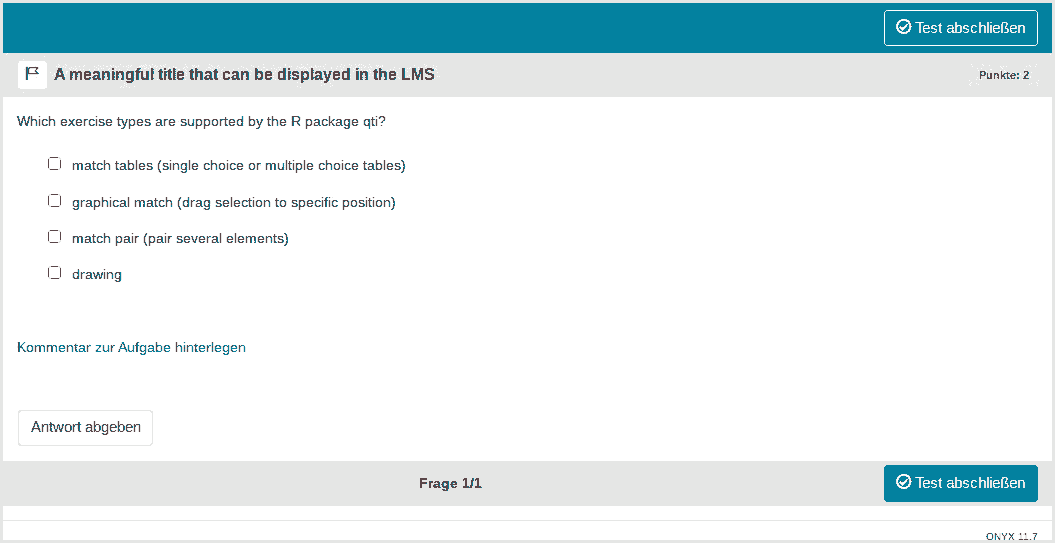
\includegraphics[width=1\textwidth,height=\textheight]{images/multiplechoice-complex.jpg}
\caption{\label{mpc2opal}More complex multiple choice task rendered in OPAL}
\end{figure}

\section{YAML attributes}\label{YAML-attributes-1}

\noindent\textbf{type}\label{type-1}

Has to be \texttt{multiplechoice} or \texttt{mpc} or \texttt{mchoice} (compatible with \texttt{exams} package).

\noindent\textbf{identifier}\label{identifier-1}

This is the ID of the task, useful for later data analysis of results. The default is the file name. If you are doing extensive data analysis later on, it makes sense to specify a meaningful identifier. In all other cases, the file name should be fine.

\noindent\textbf{title}\label{title-1}

Title of the task. Can be displayed to students depending on the learning management system settings. The default is the file name.

\noindent\textbf{shuffle}\label{shuffle-1}

If \texttt{true}, randomizes the order of the choices. Defaults to \texttt{true}. Only in rare occasions it makes sense to have a strict order of choices (setting shuffle to \texttt{false}).

\noindent\textbf{orientation}\label{orientation-1}

Should the items be displayed in \texttt{vertical} or \texttt{horizontal} mode? Default is \texttt{vertical}.

\noindent\textbf{points}\label{points-1}

How many points are given for the whole task. Default is the number of choices times 0.5. The points \(p\) are divided by the number of choices \(c\) and then distributed over all choices. A correct choice will get the student +\(p/c\), an incorrect choice -\(p/c\). Witout such a procedure, a student could always select all answers and get the maximum number of points. See also the section \ref{some-advice-on-multiple-choice-tasks} \hyperref[some-advice-on-multiple-choice-tasks]{Some advice on multiple choice tasks}.

\section{Feedback}\label{feedback-1}

Feedback can be provided with the section

\begin{itemize}
\tightlist
\item
  \textbf{\# feedback} (general feedback, displayed every time, without conditions)
\item
  \textbf{\# feedback+} (only provided if student reaches all points)
\item
  \textbf{\# feedback-} (only provided if student does not reach all points)
\end{itemize}

\section{List of answers as a variable}\label{list-of-answers-as-a-variable-1}

For more complex tasks the list of answers is often just available as a variable. In this case you can use the helper function \texttt{mdlist} to convert the vector into a markdown list:

\begin{Shaded}
\begin{Highlighting}[]
\FunctionTok{mdlist}\NormalTok{(}\FunctionTok{c}\NormalTok{(}\StringTok{"dropdown list"}\NormalTok{, }\StringTok{"programming language evaluation"}\NormalTok{, }\StringTok{"numeric gap"}\NormalTok{), }
       \AttributeTok{solutions =} \FunctionTok{c}\NormalTok{(}\DecValTok{1}\NormalTok{, }\DecValTok{3}\NormalTok{))}
\NormalTok{[}\DecValTok{1}\NormalTok{] }\StringTok{"{-} *dropdown list*}\SpecialCharTok{\textbackslash{}n}\StringTok{{-} programming language evaluation}\SpecialCharTok{\textbackslash{}n}\StringTok{{-} *numeric gap*"}
\end{Highlighting}
\end{Shaded}

\section{Some advice on multiple choice tasks}\label{some-advice-on-multiple-choice-tasks}

A multiple-choice task can always be converted into multiple single-choice questions with true/false or yes/no options. From a psychometric standpoint, both types of tasks share the same drawbacks, primarily due to the potential for guessing. Consequently, they should be avoided when possible. Generally, their psychometric properties are inferior to those of numeric or string-based gap tasks that assess similar content.

However, there are scenarios where forced-choice tasks are necessary. For example, presenting several statistical analyses and asking students to determine whether the results are statistically significant is a valuable task. Even in such cases, a multiple-choice format may not be the best option. Better alternatives include single-choice questions, dropdowns, or match tables. A multiple-choice question can often be restructured into several single-choice or dropdown questions with yes/no options. This may be cumbersome for longer multiple-choice lists, for which a match table with yes/no options can be a more convenient solution.

The main advantage of these alternative formats is that they require students to make explicit choices. In a multiple-choice task where all options are incorrect, a student could earn full points simply by not making any selections---effectively getting credit without engaging with the question. To avoid this, multiple-choice tasks must balance the distribution of correct and incorrect options, which is not necessary for single-choice, dropdown, or match table formats.

While multiple-choice tasks are supported, we strongly advise against using them whenever possible in favor of more robust alternatives.

\chapter{Gap tasks}\label{gap-tasks}

In this task format, candidates are required to fill in one or more gaps. We believe this method is one of the most effective ways to assess students' abilities, as it reduces the likelihood of guessing compared to multiple-choice questions. Emphasizing gap-fill tasks often leads to more reliable assessment outcomes.

Our package allows for the integration of both textual and numeric responses within a single task, offering instructors greater flexibility in designing assessments.

\section{Minimum version}\label{minimum-version-2}

A minimum template is automatically created when you initiate an \texttt{rqti} project through RStudio. Alternatively, it can be added by clicking on \texttt{New\ file\ \textrightarrow{}\ R\ Markdown\ \textrightarrow{}\ From\ Template}. The \texttt{rqti} templates end with \texttt{\{rqti\}}. Here we look at the templates \texttt{gap\ (simple)} and \texttt{gap\ (complex)}.

The minimum you need to provide is the \texttt{type:\ gap} (or the equivalent \texttt{type:\ cloze}) in the YAML-section and some text, where at least one gap is used, in a section called \textbf{\#question}. Furthermore, when employing helper functions from the \texttt{rqti} package, it is essential to ensure its prior loading.

\begin{Shaded}
\begin{Highlighting}
---
type: gap
knit: rqti::render_qtijs
---

```{r, preparation}
library(rqti)
```

```{r, data}
iq <- round(rnorm(10, 100, 15))
mean_iq <- mean(iq)
```

# question

## numeric gaps

IQ Tests are standardized to have a mean value of <<100>>.

You conducted an IQ test for 10 persons and found the following values:

`r iq`

What is the mean value of these IQ values? `r gap_numeric(mean(iq))`

See `?gap_numeric` for more options (e.g. tolerance).

## text gaps

The original IQ test was developed by `r gap_text(c("Alfred Binet", "Binet", "A.
Binet"))` in the early <<20th>> century with the intention of identifying
students who might need extra assistance.

See `?gap_text` for more options (e.g. tolerance).

# feedback

1. IQ Tests are standardized to have a mean of 100.
1. The correct mean value for `r iq` is `r mean_iq`.
1. The original IQ test was developed by Alfred Binet.
1. It was in the 20th century.
\end{Highlighting}
\end{Shaded}

Clicking on the Knit-button will produce the output in Figure \ref{gap1qtijs}.

\begin{figure}
\centering
\includegraphics[width=1\textwidth,height=\textheight]{images/xml/gap-simple.jpg}
\caption{\label{gap1qtijs}Simple gap task rendered in qtijs}
\end{figure}

\noindent Alternatively, change the knit parameter to \texttt{knit:\ rqti::render\_opal} (see Chapter \ref{working-with-the-opal-api} \href{api_opal.html}{Working with the OPAL API}) to upload to OPAL directly, producing the output in Figure \ref{gap1opal}.

\begin{figure}
\centering
\includegraphics[width=1\textwidth,height=\textheight]{images/gap-simple.jpg}
\caption{\label{gap1opal}Simple gap task rendered in OPAL}
\end{figure}

There are two ways to create a gap in an Rmd file:

\begin{itemize}
\tightlist
\item
  Put the correct answer between \texttt{\textless{}\textless{}} \ldots{} \texttt{\textgreater{}\textgreater{}}. Example: \texttt{\textless{}\textless{}3.14\textgreater{}\textgreater{}} or \texttt{\textless{}\textless{}sometext\textgreater{}\textgreater{}}
\item
  use the helper functions \texttt{?gap\_numeric} and \texttt{?gap\_text} (see Sections \ref{gaptext} \hyperref[gaptext]{Helper function gap text}, \ref{gapnumeric} \hyperref[gapnumeric]{Helper function gap numeric})
\end{itemize}

We generally recommend to use the helper function as it allows to set additional parameters.

By default, 1 point can be reached for each gap (specify \texttt{points} in the helper function to your needs). The total number of points for completing a task is defined as the sum of points of all gaps.

Note that in this example, a feedback section was also provided. The feedback is
optional, but usually it is a good idea to give some explanation for students. In gap tasks the feedback refers to the whole task, not to a specific gap. Group your feedback into appropriate sections, which can be opened/closed for better user experience (use \texttt{\textless{}details\textgreater{}} and \texttt{\textless{}summary\textgreater{}} html tags).

A great way to do this is to use \texttt{\textless{}details\textgreater{}} and \texttt{\textless{}summary\textgreater{}} html tags:

\begin{Shaded}
\begin{Highlighting}[]
\DataTypeTok{\textless{}}\KeywordTok{details}\DataTypeTok{\textgreater{}\textless{}}\KeywordTok{summary}\DataTypeTok{\textgreater{}}\NormalTok{Question1}\DataTypeTok{\textless{}/}\KeywordTok{summary}\DataTypeTok{\textgreater{}}
\NormalTok{  Provide Feedback for Question 1}
\DataTypeTok{\textless{}/}\KeywordTok{details}\DataTypeTok{\textgreater{}}
\DataTypeTok{\textless{}}\KeywordTok{details}\DataTypeTok{\textgreater{}\textless{}}\KeywordTok{summary}\DataTypeTok{\textgreater{}}\NormalTok{Question 2}\DataTypeTok{\textless{}/}\KeywordTok{summary}\DataTypeTok{\textgreater{}}
\NormalTok{  Provide Feedback for Question 2}
\DataTypeTok{\textless{}/}\KeywordTok{details}\DataTypeTok{\textgreater{}}
\end{Highlighting}
\end{Shaded}

will render as:

\noindent\textrightarrow{} Question 1\\
\noindent\textrightarrow{} Question 2\\

By clicking on the arrows, the details will unfold.

\section{More control}\label{more-control-2}

If you want to have more fine-grained control, consider the RMD template \texttt{gap\ (complex)}, which uses more YAML attributes and more complex calls of the helper functions.

\begin{Shaded}
\begin{Highlighting}
---
type: gap # type of exercise
knit: rqti::render_qtijs # if you do not want our preview renderer, remove this
identifier: gap001 # think twice about this id for later data analysis!
title: A meaningful title that can be displayed in the LMS
---

```{r, preparation}
library(rqti)
```

```{r, data}
iq <- round(rnorm(10, 100, 15))
mean_iq <- mean(iq)
```

# question

## numeric gaps

IQ Tests are standardized to have a mean value of <<100>>.

You conducted an IQ test for 10 persons and found the following values:

`r iq`

What is the mean value of these IQ values? `r gap_numeric(mean(iq))`

The same question, but now with a tolerance of +-5: `r gap_numeric(mean(iq),
tolerance = 5)`

The parameter `tolerance_type` determines how the tolerance is calculated.

The same question, but now with a relative tolerance of +-5%: `r
gap_numeric(mean(iq), tolerance = 5, tolerance_type = "relative")`

## text gaps

The original IQ test was developed by `r gap_text(c("Alfred Binet", "Binet", "A.
Binet"))` in the early 20th century with the intention of identifying students
who might need extra assistance. Over the years, IQ tests have evolved, and
various versions exist today, such as the WAIS, standing for `r
gap_text("Wechsler", case_sensitive = F, tolerance = 2)` Adult Intelligence
Scale, and the <<Stanford>>-Binet Intelligence Scales.

Please be advised that OPAL has introduced a new attribute for text
gaps—`tolerance`—which now accommodates considerations for spelling errors. It
is crucial to restrict the use of this attribute to the OPAL Learning Management
System (LMS), as it may not be compatible with other Learning Management
Systems. Furthermore, it is important to note that employing this attribute will
result in the XML files being rendered invalid according to the QTI standard.

# feedback

1. IQ Tests are standardized to have a mean of 100.
1. The correct mean value for `r iq` is `r mean_iq`.
1. The original IQ test was developed by Alfred Binet.
1. WAIS: W stands for Wechsler
1. It is the Stanford-Binet Intelligence Scales.

<!-- If you prefer specific feedback for correct and incorrect solution, delete
the general feedback section and uncomment everything starting from the next
line:

# feedback+

Nice. (Only displayed when the solution is correct.)

# feedback-

Try again. (Only displayed if the solution is not correct.)
-->
\end{Highlighting}
\end{Shaded}

In OPAL this renders as shown in Figure \ref{gap2opal}.

\begin{figure}
\centering
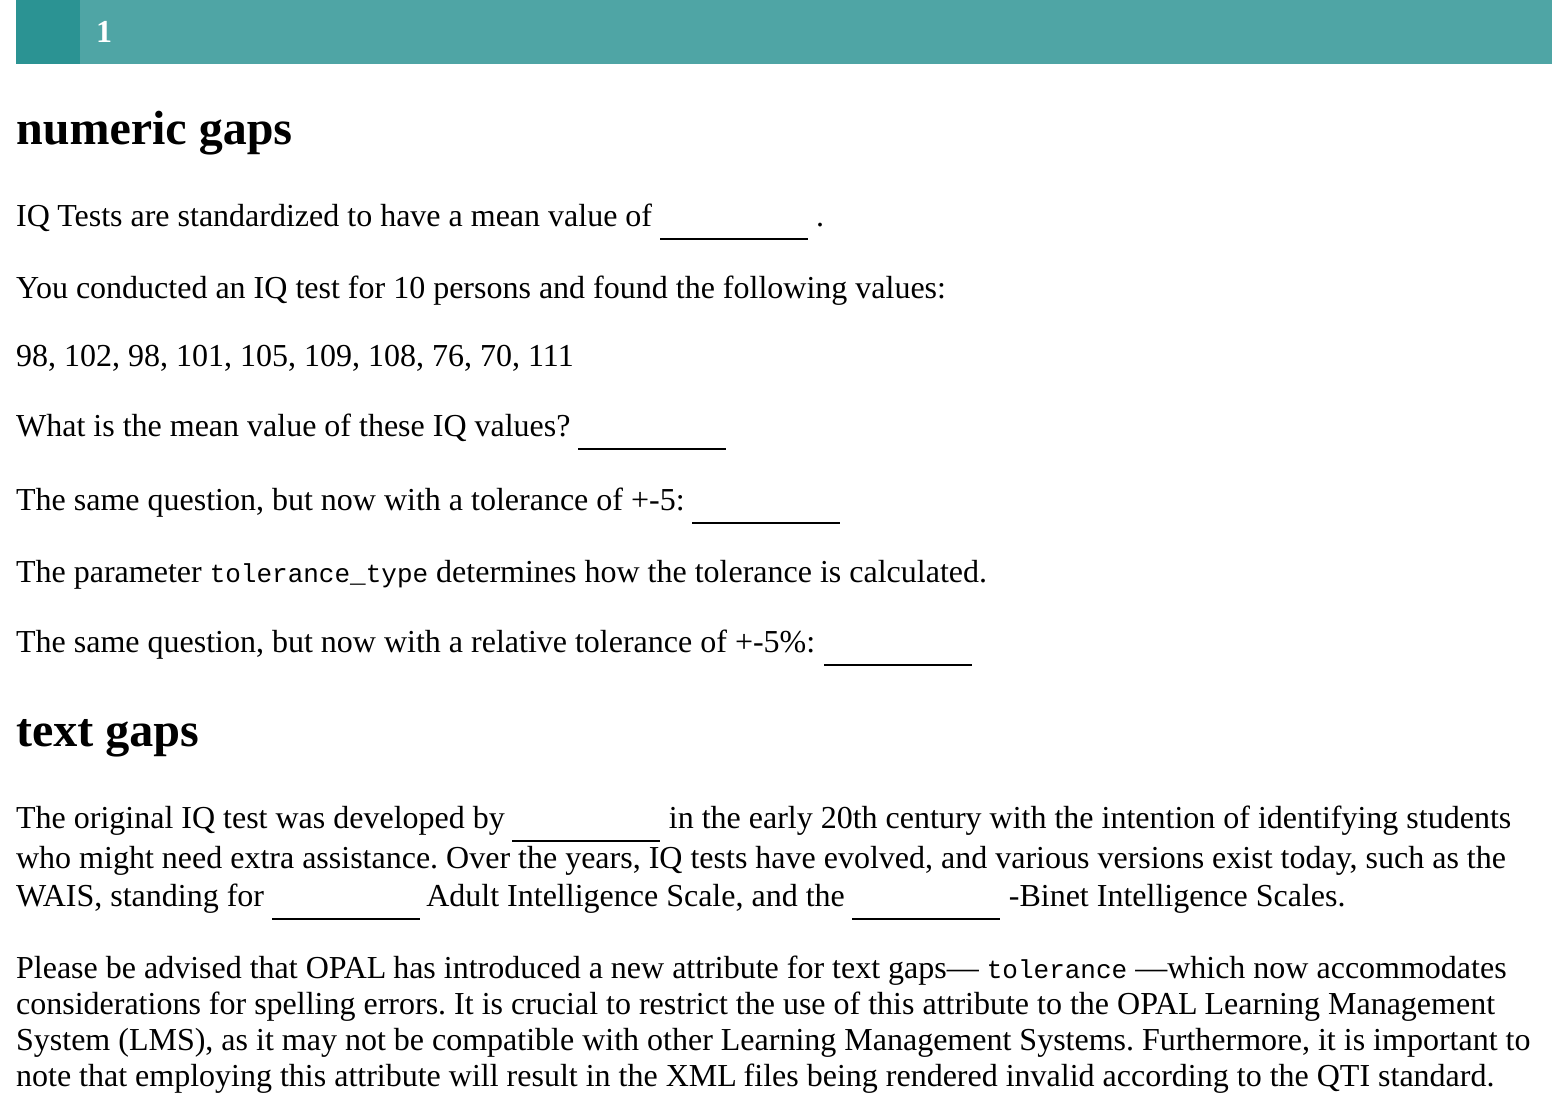
\includegraphics[width=1\textwidth,height=\textheight]{images/gap-complex.jpg}
\caption{\label{gap2opal}Preview of complex gap task in OPAL}
\end{figure}

\section{YAML attributes}\label{YAML-attributes-2}

\noindent\textbf{type}\label{type-2}

Has to be \texttt{gap} or \texttt{cloze}.
\newpage
\noindent\textbf{identifier}\label{identifier-2}

This is the ID of the task, useful for later data analysis of results. The default is the file name. If you are doing extensive data analysis later on it makes sense to
specify a meaningful identifier. In all other cases, the file name should be
fine.

\noindent\textbf{title}\label{title-2}

Title of the task. Can be displayed to students depending on
the learning management system settings. Default is the file name.

\section{Feedback}\label{feedback-2}

Feedback can be provided with the section

\begin{itemize}
\tightlist
\item
  \textbf{\# feedback} (general feedback, displayed every time, without conditions)
\item
  \textbf{\# feedback+} (only provided if student reaches all points)
\item
  \textbf{\# feedback-} (only provided if student does not reach all points)
\end{itemize}

\section{\texorpdfstring{Helper function \texttt{gap\_numeric}}{Helper function gap\_numeric}}\label{gapnumeric}

This helper function generates a formatted string to describe a gap in Rmd content, specifically where the expected answer is numeric. It supports numerous attributes, with the most useful ones demonstrated in the following example:

\begin{Shaded}
\begin{Highlighting}[]
\NormalTok{gap1 }\OtherTok{\textless{}{-}} \FunctionTok{gap\_numeric}\NormalTok{(}\AttributeTok{solution =} \FloatTok{1.4}\NormalTok{, }\AttributeTok{tolerance =} \DecValTok{10}\NormalTok{, }\AttributeTok{tolerance\_type =} \StringTok{"relative"}\NormalTok{,}
                    \AttributeTok{points =} \DecValTok{5}\NormalTok{, }\AttributeTok{response\_identifier =} \StringTok{"mean\_value"}\NormalTok{,}
                    \AttributeTok{include\_lower\_bound =} \ConstantTok{TRUE}\NormalTok{, }\AttributeTok{include\_upper\_bound =} \ConstantTok{TRUE}\NormalTok{,}
                    \AttributeTok{expected\_length =} \DecValTok{10}\NormalTok{, }\AttributeTok{placeholder =} \StringTok{"put mean value here"}\NormalTok{)}
\FunctionTok{cat}\NormalTok{(gap1)}
\SpecialCharTok{\textless{}}\NormalTok{gap}\SpecialCharTok{\textgreater{}}\NormalTok{\{solution}\SpecialCharTok{:}\NormalTok{ [}\FloatTok{1.4}\NormalTok{], tolerance}\SpecialCharTok{:} \FloatTok{10.0}\NormalTok{, tolerance\_type}\SpecialCharTok{:}\NormalTok{ relative, points}\SpecialCharTok{:} \FloatTok{5.0}\NormalTok{,}
\NormalTok{response\_identifier}\SpecialCharTok{:}\NormalTok{ mean\_value, include\_lower\_bound}\SpecialCharTok{:}\NormalTok{ yes,}
\NormalTok{include\_upper\_bound}\SpecialCharTok{:}\NormalTok{ yes, expected\_length}\SpecialCharTok{:} \FloatTok{10.0}\NormalTok{, placeholder}\SpecialCharTok{:}\NormalTok{ put mean value here,}
\NormalTok{type}\SpecialCharTok{:}\NormalTok{ numeric\}}\SpecialCharTok{\textless{}}\ErrorTok{/}\NormalTok{gap}\SpecialCharTok{\textgreater{}}
\end{Highlighting}
\end{Shaded}

As you can see, YAML is ultimately used as the input, so you do not necessarily need the helper function. Still, for most users, it is more convenient to have a dedicated R function to simplify the workflow.

Let us now look at the argument list of \texttt{gap\_numeric}:

\noindent\textbf{solution}\label{solution}

Correct numeric answer.

\noindent\textbf{tolerance}\label{tolerance}

Defines the range of values within which an answer is deemed correct.

\noindent\textbf{tolerance\_type}\label{tolerance_type}

Defines how the tolerance is calculated. For instance, if the solution is 50 and the tolerance is 10:

\begin{itemize}
\tightlist
\item
  Setting \texttt{tolerance\_type} to \texttt{relative} results in a correct answer range from 45 to 55 (50 ± 10\%).
\item
  Setting it to \texttt{absolute} creates a range from 40 to 60 (50 ± 10).
\end{itemize}

\noindent\textbf{points}\label{points-2}

The number of points for this gap. Default is 1.

\noindent\textbf{response\_identifier}\label{response_identifier}

This is the ID of the gap, useful for later data analysis. The default has the format ``response\_1'', ``response\_2''. If you are doing extensive data analysis later on, it makes sense to specify a meaningful identifier.

\noindent\textbf{include\_lower\_bound}\label{include_lower_bound}

Specifies whether the lower bound is included in the tolerance interval.

\noindent\textbf{inclue\_upper\_bound}\label{inclue_upper_bound}

Specifies whether the upper bound is included in the tolerance interval.

\noindent\textbf{expected\_length}\label{expected_length}

Specifies the size of the text input field in the content delivery engine. This value is not directly assigned, it is calculated based on the number of symbols in the solution value. Browsers display the input field length inconsistently, but we have endeavored to establish sensible defaults.

\noindent\textbf{placeholder}\label{placeholder}

Text displayed in the gap, before an answer is attempted. Can be used for hints (e.g.~\emph{numbers only}).

\section{\texorpdfstring{Helper function \texttt{gap\_text}}{Helper function gap\_text}}\label{gaptext}

This helper function is designed to generate a formatted string describing a gap in Rmd content, where the answer is a string:

\begin{Shaded}
\begin{Highlighting}[]
\NormalTok{gap2 }\OtherTok{\textless{}{-}} \FunctionTok{gap\_text}\NormalTok{(}\FunctionTok{gap\_text}\NormalTok{(}\FunctionTok{c}\NormalTok{(}\StringTok{"Bildungsportal Sachsen"}\NormalTok{, }\StringTok{"Bildungs Portal Sachsen"}\NormalTok{),}
                          \AttributeTok{tolerance =} \DecValTok{4}\NormalTok{, }\AttributeTok{case\_sensitive =} \ConstantTok{FALSE}\NormalTok{, }
                          \AttributeTok{placeholder =} \StringTok{"text without special characters"}\NormalTok{,}
                          \AttributeTok{expected\_length =} \DecValTok{25}\NormalTok{))}
\end{Highlighting}
\end{Shaded}

The argument list of \texttt{gap\_text} is similar to \texttt{gap\_numeric}, but most learning management systems do not handle tolerance by default. However, OPAL has implemented a method to manage tolerance, which works reasonably well. Keep in mind that this functionality only works on OPAL and does not comply with the QTI standard. Let us look at all available parameters of \texttt{gap\_text}:

\noindent\textbf{solution}\label{solution-1}

Determines a string vector of values that are considered as correct answers.

\noindent\textbf{tolerance (works only in LMS OPAL)}\label{tolerance-works-only-in-lms-opal}

Defines how many characters will be taken into account to tolerate spelling mistakes. The exact algorithm of OPAL is unclear.

\noindent\textbf{case\_sensitive (works only in LMS OPAL)}\label{case_sensitive-works-only-in-lms-opal}

Determines whether the evaluation of the correct answer is case sensitive. Default is \texttt{FALSE}.

\noindent\textbf{points}\label{points-3}

The number of points for this gap. Default is 1.

\noindent\textbf{response\_identifier}\label{response_identifier-1}

This is the ID of the gap, useful for later data analysis. The default has the format ``response\_1'', ``response\_2''. If you are doing extensive data analysis later on, it makes sense to specify a meaningful identifier.

\noindent\textbf{expected\_length}\label{expected_length-1}

Specifies the size of the text input field in the content delivery engine. The default value is calculated based on the number of symbols in the solution value. Browsers display the input field length inconsistently, but we have endeavored to establish sensible defaults. Please adjust to your needs.

\noindent\textbf{placeholder}\label{placeholder-1}

Text displayed in the gap, before an answer is attempted. Can be used for hints (e.g.~\emph{numbers only}).

\section{Some advice on gap tasks}\label{some-advice-on-gap-tasks}

Gap tasks are generally foolproof, offering an ideal format by minimizing guessing and often presenting a reasonably high level of difficulty. Numeric tasks, involving calculations that are typically not guessable, are especially effective. While crafting text gaps may be more intricate, the option to offer multiple alternative solutions and leverage OPAL to accommodate spelling errors enhances their versatility. Nevertheless, it is important to note that, like any task, gap tasks can be poorly designed, so be mindful in their creation.

As mentioned earlier, numeric and text gaps can be combined in a single task, making them quite versatile. In fact, the flexibility of gaps allows for the integration of various task types within a single task. For instance, to incorporate single-choice questions alongside gaps, you can use a numeric gap for the single-choice question and include the answer options directly in the question. For example, ``Fill in the blank: \_\_\_\_ (0 = not significant, 1 = significant)''. This approach enables you to use gaps for many types of questions, highlighting their exceptional adaptability.

\chapter{Dropdown tasks}\label{dropdown-tasks}

In this type of task, the candidate has to select an element form a dropdown-list. Note that our package implements dropdowns as \emph{entry}-objects because this is essentially what dropwdowns are. Several dropdowns can be combined in a single task, but a combination with numeric and text entries (gaps) is not possible; mainly due to limitations on the site of learning managment systems.

\section{Minimum version}\label{minimum-version-3}

A minimum template is automatically created when you initiate an \texttt{rqti} project through RStudio. Alternatively, it can be added by clicking on \texttt{New\ file\ \textrightarrow{}\ R\ Markdown\ \textrightarrow{}\ From\ Template}. The \texttt{rqti} templates end with \texttt{\{rqti\}}. Here we look at the templates \texttt{dropdown\ (simple)} and \texttt{dropdown\ (complex)}.

The minimum you need to provide is the \texttt{type:\ dropdown} (or the equivalent \texttt{type:\ dd}) in the YAML-section and some text, where at least one gap is formed as a dropdown-element, in a section called \textbf{\#question}. Furthermore, when employing helper functions from the \texttt{rqti} package, it is essential to ensure its prior loading.

\begin{Shaded}
\begin{Highlighting}
---
type: dropdown
knit: rqti::render_qtijs
---

```{r echo=F}
library(rqti)
```

# question

The philosophy of the rqti package is <<do one thing and do it well|one for
all>>.

Under the hood, the rqti package uses `r dropdown(c("S4 OOP", "S3 OOP", "no
OOP", "R6 OOP"))`.

# feedback

The package `rqti` is specialized for producing xml rqti files so "do one thing
and do it well" is more appropriate. Under the hood we use S4 OOP.
\end{Highlighting}
\end{Shaded}

Knitting via the Knit-Button to qtijs, this task renders as shown in Figure \ref{dd1qtijs}.

\begin{figure*}
\centering
\includegraphics[width=1\textwidth,height=\textheight]{images/xml/dropdown-simple.jpg}
\caption{\label{dd1qtijs}Simple dropdown task rendered in qtijs}
\end{figure*}

\noindent Alternatively, change the knit parameter to \texttt{knit:\ rqti::render\_opal} (see Chapter \ref{working-with-the-opal-api} \href{api_opal.html}{Working with the OPAL API}) to upload to OPAL directly, producing the output in Figure \ref{dd1opal}.

\begin{figure*}
\centering
\includegraphics[width=1\textwidth,height=\textheight]{images/dropdown-simple.jpg}
\caption{\label{dd1opal}Simple dropdown task rendered in OPAL}
\end{figure*}
\newpage
There are two ways to specify a dropdown-element in Rmd content:

\begin{itemize}
\tightlist
\item
  Put the correct answer inside \texttt{\textless{}\textless{}} \ldots{} \texttt{\textgreater{}\textgreater{}} (or the equivalent \texttt{\textless{}gap\textgreater{}} \ldots{} \texttt{\textless{}/gap\textgreater{}}). Example: \texttt{\textless{}\textless{}element1\textbar{}element2\textbar{}element3\textgreater{}\textgreater{}}
\item
  use the helper function \texttt{?dropdown} (also see section \ref{helper-function-dropdown} \hyperref[helper-function-dropdown]{Helper function dropdown})
\end{itemize}

By default, 1 point can be reached for each dropdown (specify \texttt{points} to your needs). The total number of points for completing a task is defined as the sum of points of all dropdowns.

Note that in this example, a feedback section was also provided. The feedback is
optional, but usually it is a good idea to give some explanation for students. In dropdown tasks the feedback refers to the whole task, not to a specific dropdown. Group your feedback into appropriate sections, which can be opened/closed for better user experience. A great way to do this is to use \texttt{\textless{}details\textgreater{}} and \texttt{\textless{}summary\textgreater{}} html tags:

\begin{Shaded}
\begin{Highlighting}[]
\DataTypeTok{\textless{}}\KeywordTok{details}\DataTypeTok{\textgreater{}\textless{}}\KeywordTok{summary}\DataTypeTok{\textgreater{}}\NormalTok{Question1}\DataTypeTok{\textless{}/}\KeywordTok{summary}\DataTypeTok{\textgreater{}}
\NormalTok{  Provide Feedback for Question 1}
\DataTypeTok{\textless{}/}\KeywordTok{details}\DataTypeTok{\textgreater{}}
\DataTypeTok{\textless{}}\KeywordTok{details}\DataTypeTok{\textgreater{}\textless{}}\KeywordTok{summary}\DataTypeTok{\textgreater{}}\NormalTok{Question 2}\DataTypeTok{\textless{}/}\KeywordTok{summary}\DataTypeTok{\textgreater{}}
\NormalTok{  Provide Feedback for Question 2}
\DataTypeTok{\textless{}/}\KeywordTok{details}\DataTypeTok{\textgreater{}}
\end{Highlighting}
\end{Shaded}

will render as:

\noindent\textrightarrow{} Question 1\\
\noindent\textrightarrow{} Question 2\\

By clicking on the arrows, the details will unfold.

\section{More control}\label{more-control-3}

If you want to have more fine-grained control, consider the RMD template \texttt{dropdown\ (complex)}, which uses more YAML attributes and a more complex use of the helper function \texttt{dropdown}.

\begin{Shaded}
\begin{Highlighting}
---
type: dd # type of exercise
knit: rqti::render_qtijs # if you do not want our preview renderer, remove this
identifier: dd001 # think twice about this id for later data analysis!
title: A meaningful title that can be displayed in the LMS
---

```{r echo=F}
library(rqti)
```

# question

The philosophy of the rqti package is <<do one thing and do it well|one for
all>>.

Under the hood, the rqti package uses `r dropdown(c("no OOP" = "no OOP", "S4" =
"S4 OOP", "S3" = "S3 OOP", "R6" = "R6 OOP"), solution_index = 2, points = 2,
response_identifier = "OOP_task")`.

# feedback

The package `rqti` is specialized for producing xml rqti files so "do one thing
and do it well" is more appropriate. Under the hood we use S4 OOP.
\end{Highlighting}
\end{Shaded}

This renders in OPAL as shown in Figure \ref{dd2opal}. In reality, there is not much to observe here since the relevant settings are only visible during interaction with the exercise. The only changes are to the title and points.

\begin{figure*}
\centering
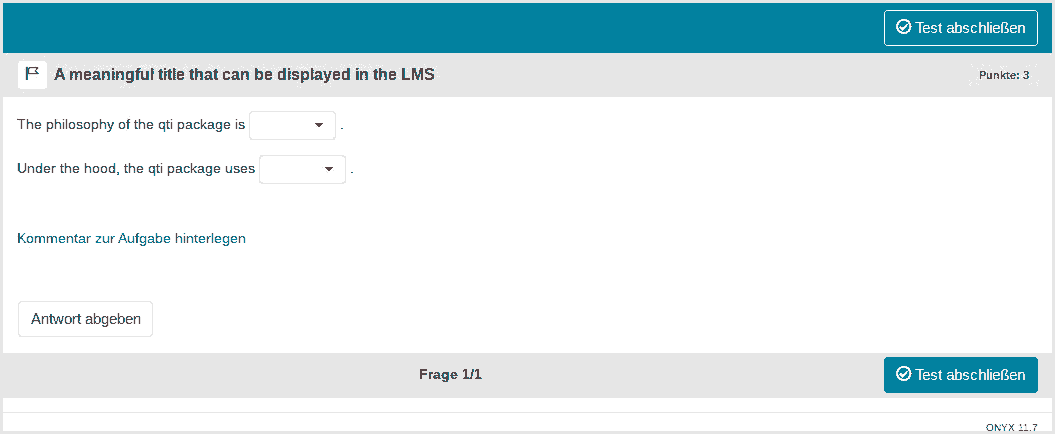
\includegraphics[width=1\textwidth,height=\textheight]{images/dropdown-complex.jpg}
\caption{\label{dd2opal}More complex dropdown task rendered in OPAL}
\end{figure*}

Since dropdowns are primarily defined through helper functions, there are few relevant YAML attributes.

\section{YAML attributes}\label{YAML-attributes-3}

\noindent\textbf{type}\label{type-3}

Has to be \texttt{dropdown} or \texttt{dd}.

\noindent\textbf{identifier}\label{identifier-3}

This is the ID of the task, useful for later data analysis of results. The default is the file name. If you are doing extensive data analysis later on it makes sense to specify a meaningful identifier. In all other cases, the file name should be fine.

\noindent\textbf{title}\label{title-3}

Title of the task. Can be displayed to students depending on the learning management system settings. Default is the file name.

\section{Feedback}\label{feedback-3}

Feedback can be provided with the section

\begin{itemize}
\tightlist
\item
  \textbf{\# feedback} (general feedback, displayed every time, without conditions)
\item
  \textbf{\# feedback+} (only provided if student reaches all points)
\item
  \textbf{\# feedback-} (only provided if student does not reach all points)
\end{itemize}

\section{\texorpdfstring{Helper function \texttt{dropdown}}{Helper function dropdown}}\label{helper-function-dropdown}

This helper function is used to generate a formatted string describing a dropdown in Rmd content:

\begin{Shaded}
\begin{Highlighting}[]
\NormalTok{choices }\OtherTok{\textless{}{-}} \FunctionTok{c}\NormalTok{(}\StringTok{"s4"} \OtherTok{=} \StringTok{"S4 OOP"}\NormalTok{, }\StringTok{"s3"} \OtherTok{=} \StringTok{"S3 OOP"}\NormalTok{, }\StringTok{"none"} \OtherTok{=} \StringTok{"no OOP"}\NormalTok{, }\StringTok{"r6"} \OtherTok{=} \StringTok{"R6 OOP"}\NormalTok{)}
\NormalTok{oop\_task }\OtherTok{\textless{}{-}} \FunctionTok{dropdown}\NormalTok{(}\AttributeTok{choices =}\NormalTok{ choices, }\AttributeTok{solution =} \StringTok{"S4 OOP"}\NormalTok{,}
                     \AttributeTok{response\_identifier =} \StringTok{"OOP\_task"}\NormalTok{)}
\end{Highlighting}
\end{Shaded}

The arguments of the \texttt{dropdown} function are:

\noindent\textbf{choices}\label{choices}

Elements of dropdown. If you use a named vector, the names will be used as identifiers. This is useful for later data analysis and is generally adviced.

\noindent\textbf{solution\_index}\label{solution_index}

The index of the correct choice as a numeric. Default is 1, meaning that you can simply put the correct element as the first one in the vector \texttt{choices}.

\noindent\textbf{points}\label{points-4}

The number of points for the task. Default is 1.

\noindent\textbf{shuffle}\label{shuffle-2}

If \texttt{TRUE}, randomizes the order of the choices. Defaults to \texttt{TRUE}. Only in rare occasions it makes sense to have a strict order of choices (setting shuffle to \texttt{FALSE}).

\noindent\textbf{response\_identifier}\label{response_identifier-2}

This is the ID of the dropdown-element, useful for later data analysis of results. The default has the format ``response\_1'', ``response\_2'', \ldots{}``response\_n'' for several dropdowns. If you are doing extensive data analysis later on, it makes sense to specify a more meaningful identifier.

\section{Some advice on dropdown tasks}\label{some-advice-on-dropdown-tasks}

Dropdown tasks are forced choice items, so are equivalent to single choice tasks. The advantage is that they can be placed in between other text and several of them can be used in a single task. Still, they suffer from the same problems as \href{singlechoice.html}{single choice tasks}.

\chapter{Essay tasks}\label{essay-tasks}

This is a standard essay task that allows students to provide a comprehensive response in an open field. Unlike other types of assessments, essays cannot be graded automatically by default. However, if AI is integrated, it can assist in evaluating the responses.

\section{Minimum version}\label{minimum-version-4}

A minimum template is automatically created when you initiate an \texttt{rqti} project through RStudio. Alternatively, it can be added by clicking on \texttt{New\ file\ \textrightarrow{}\ R\ Markdown\ \textrightarrow{}\ From\ Template}. The \texttt{rqti} templates end with \texttt{\{rqti\}} Here we look at the templates \texttt{essay\ (simple)} and \texttt{essay\ (complex)}.

The minimum you need to provide is the \texttt{type:\ essay} in the YAML-section and some text as a task description in a section called \textbf{\#question}:

\begin{Shaded}
\begin{Highlighting}
---
type: essay # type of exercise
knit: rqti::render_qtijs # if you do not want our preview renderer, remove this
---

# question

What are the advantages and disadvantages of the `rqti` package as compared to
the `exams` package?

# feedback

The rqti package can only export to the QTI format, which makes it less general
than the `exams` package. But the rqti package supports more exercise types, can
preview xml files, supports the OPAL API and has an extensible core architecture
based on S4 OOP.
\end{Highlighting}
\end{Shaded}

Knitting via the Knit-Button to qtijs, this task renders as shown in Figure \ref{essay1qtijs}.

\begin{figure*}
\centering
\includegraphics[width=1\textwidth,height=\textheight]{images/xml/essay-simple.jpg}
\caption{\label{essay1qtijs}Simple essay erxercise rendered by qtijs}
\end{figure*}

\noindent Alternatively, change the knit parameter to \texttt{knit:\ rqti::render\_opal} (see \href{api_opal.html}{Working with the OPAL API}) to upload to OPAL directly, producing a very similar rendering.
%
% \begin{figure}
% \centering
% \includegraphics[width=1\textwidth,height=\textheight]{images/essay-simple.jpg}
% \caption{\label{essay1opal}Simple essay task rendered by OPAL}
% \end{figure}

Note that in this example, a feedback section was also provided. Since an open question requires manual review, only general feedback without conditions should be provided. The feedback is optional, but usually it is a good idea to give some explanation for students. Furthermore, a feedback section for essay tasks can serve as a good basis for grading student's answers. In addition the length of the feedback section is taken into account in constructing the text field and the maximum number of words. If no feedback is provided, sensible defaults are used.

\section{More control}\label{more-control-4}

If you want to have more fine-grained control, consider the RMD template \texttt{essay\ (complex)}, which uses more YAML attributes.

\begin{Shaded}
\begin{Highlighting}
---
type: essay # type of exercise
knit: rqti::render_qtijs # if you do not want our preview renderer, remove this
identifier: essay001 # think twice about this id for later data analysis!
title: A meaningful title that can be displayed in the LMS
expected_length: 30 # defines the width of the text input field
expected_lines: 3 # defines the number of lines of the text input field
words_max: 100 # how many words can be written in the text input field
words_min: 10 # the minimum number of words to send a response
data_allow_paste: false # allows to copy text from the clipboard
points: 2
---

# question

What are the advantages and disadvantages of the `rqti` package as compared to
the `exams` package?

# feedback

The rqti package can only export to the QTI format, which makes it less general
than the `exams` package. But the rqti package supports more exercise types, can
preview xml files, supports the OPAL API and has an extensible core architecture
based on S4 OOP.
\end{Highlighting}
\end{Shaded}

Which, in OPAL, renders as shown in Figure \ref{essay2opal}.

\begin{figure*}
\centering
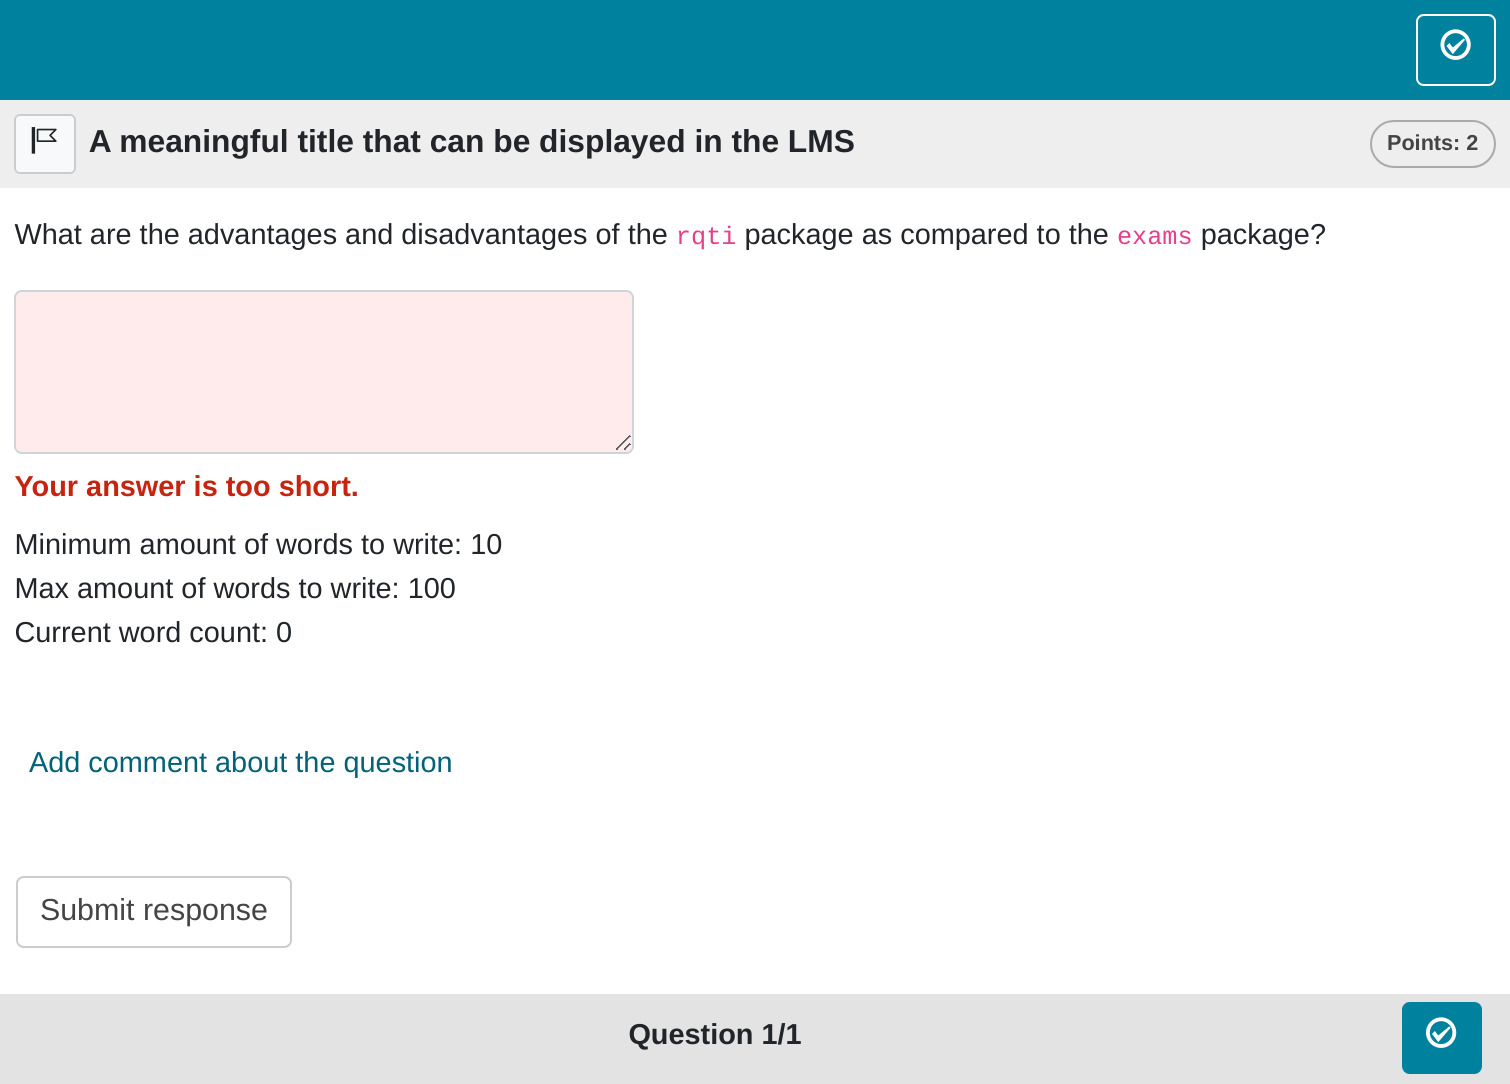
\includegraphics[width=1\textwidth,height=\textheight]{images/essay-complex.jpg}
\caption{\label{essay2opal}More complex essay task rendered in OPAL}
\end{figure*}

\section{YAML attributes}\label{YAML-attributes-4}

\noindent\textbf{type}\label{type-4}

Has to be \texttt{essay}.

\noindent\textbf{identifier}\label{identifier-4}

This is the ID of the task, useful for later data analysis of results. The default is the file name. If you are doing extensive data analysis later on it makes sense to specify a meaningful identifier. In all other cases, the file name should be fine.

\noindent\textbf{title}\label{title-4}

Title of the task. Can be displayed to students depending on the learning management system settings. Default is the file name.

\noindent\textbf{points}\label{points-5}

How many points are given for the whole task. Default is 1.

\noindent\textbf{expected\_length}\label{expected_length-2}

Defines the width of the text input field.

\noindent\textbf{expected\_lines}\label{expected_lines}

Defines the number of lines of the text input field.

\noindent\textbf{words\_max}\label{words_max}

Defines the maximum number of words that can be written by the candidate in the text input field.

\noindent\textbf{words\_min}\label{words_min}

Defines the minimum number of words that must be written by the candidate in the text input field.

\noindent\textbf{data\_allow\_paste}\label{data_allow_paste}

Determines whether the candidate is allowed to copy text from the clipboard to the text input field. Default is \texttt{false}.

\section{Feedback}\label{feedback-4}

Feedback can be provided with the section

\begin{itemize}
\tightlist
\item
  \textbf{\# feedback} (general feedback, displayed every time, without conditions)
\end{itemize}

The feedback plays an important role in essay tasks because the expected length and maximum words are calculated from the feedback section, if one is given. Providing useful feedback also defines explicit criteria for grading, so do not skip it for essay tasks, unless you have good reasons to.

Further note that it does not make sense to give conditional feedback as essay tasks have to be graded manually.

\section{Some advice on essay tasks}\label{some-advice-on-essay-tasks}

Essay tasks can be highly diagnostic, especially when instructors pose thought-provoking questions. Unfortunately, many instructors struggle with creativity and precision when crafting essay prompts, leading to vague grading criteria. To address this issue, it is recommended to always include an exemplary solution in the feedback section. This not only enhances the learning experience for students but also earns appreciation from colleagues involved in grading.

\chapter{Order tasks}\label{order-tasks}

In this type of task, the candidate must arrange a list of items in the correct order. While this task offers an engaging variation, it presents some challenges, as grading is less straightforward.

\section{Minimum version}\label{minimum-version-5}

A minimum template is automatically created when you initiate an \texttt{rqti} project through RStudio. Alternatively, it can be added by clicking on \texttt{New\ file\ \textrightarrow{}\ R\ Markdown\ \textrightarrow{}\ From\ Template}. The \texttt{rqti} templates end with \texttt{\{rqti\}}. Here we look at the templates \texttt{order\ (simple)} and \texttt{order\ (complex)}.

The minimum you need to provide is the \texttt{type:\ order} in the YAML-section and a list with at least two elements in a section called \textbf{\#question}:

\begin{Shaded}
\begin{Highlighting}
---
type: order
knit: rqti::render_qtijs
---

# question

What is the structure of an exam in QTI terms, starting from the top (the exam)
to the bottom (individual questions).

- test
- section
- item
- interaction

# feedback

For order exercises it is usually clear why the given order is correct, but you
might still want to provide a detailed feedback.
\end{Highlighting}
\end{Shaded}

Knitting via the Knit-Button to qtijs, this task renders as shown in Figure \ref{order1qtijs}.

\begin{figure}
\centering

\includegraphics[width=1\textwidth,height=\textheight]{images/xml/order-simple.jpg}
\caption{\label{order1qtijs}Simple order task rendered in qtijs}
\end{figure}

\noindent Alternatively, change the knit parameter to \texttt{knit:\ rqti::render\_opal} (see Chapter \ref{working-with-the-opal-api} \href{api_opal.html}{Working with the OPAL API}) to upload to OPAL directly, producing the output in Figure \ref{order1opal}.

\begin{figure}
\centering

\includegraphics[width=1\textwidth,height=\textheight]{images/order-simple.jpg}
\caption{\label{order1opal}Simple order task rendered in OPAL}
\end{figure}

The order of the items in the Rmd-list is considered to be the correct one.

Note that in this example, a feedback section was provided. The feedback is
optional, but usually it is a good idea to give some explanation for students.

\section{More control}\label{more-control-5}

If you want to have more fine-grained control, consider the Rmd template \texttt{order\ (complex)}, which uses more YAML attributes.

\begin{Shaded}
\begin{Highlighting}
---
type: order
knit: rqti::render_qtijs
identifier: order001 # think twice about this id for later data analysis!
title: A meaningful title that can be displayed in the LMS
# defines the scoring method, `false` means the correct order must be restored
# completely by the candidate in order to get points
points_per_answer: false
points: 2
---

# question

What is the structure of an exam in QTI terms, starting from the top (the exam)
to the bottom (individual questions).

- test
- section
- item
- interaction

# feedback

For order exercises it is usually clear why the given order is correct, but you
might still want to provide a detailed feedback.

<!-- If you prefer specific feedback for correct and incorrect solution, delete
the general feedback section and uncomment everything starting from this line:

# feedback+

Nice. (Only displayed when the solution is correct.)

# feedback-

Try again. (Only displayed if the solution is not correct.)
-->
\end{Highlighting}
\end{Shaded}

Which on OPAL renders as shown in Figure \ref{order2opal}.

\begin{figure}
\centering
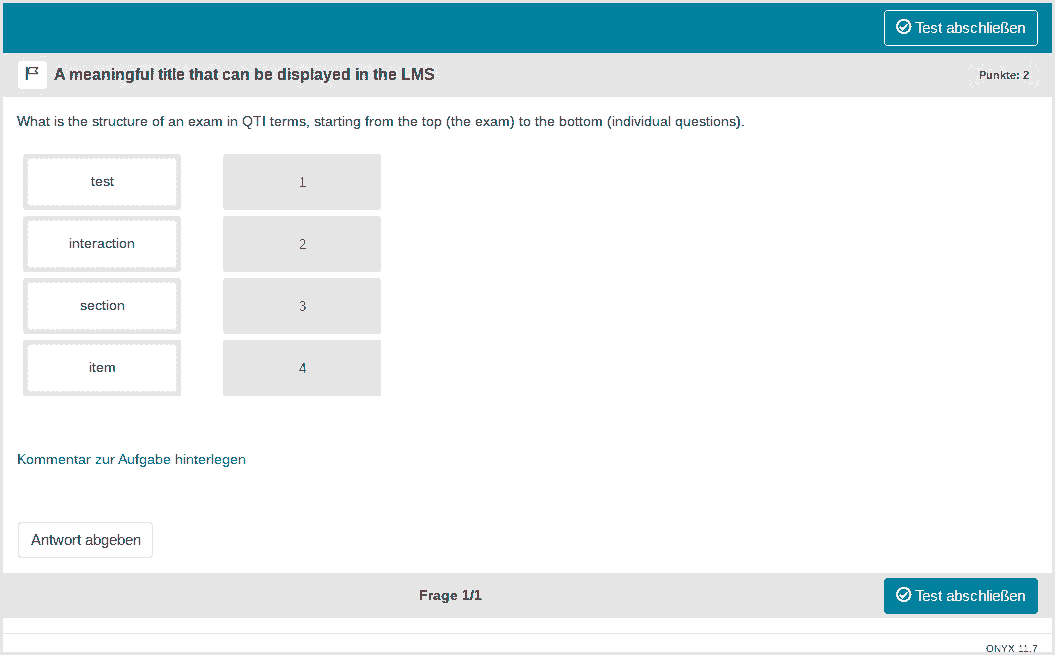
\includegraphics[width=1\textwidth,height=\textheight]{images/order-complex.jpg}
\caption{\label{order2opal}More complex order task rendered in OPAL}
\end{figure}

\section{YAML attributes}\label{YAML-attributes-5}

\noindent\textbf{type}\label{type-5}

Has to be \texttt{order}.

\noindent\textbf{identifier}\label{identifier-5}

This is the ID of the task, useful for later data analysis of results. The default is the file name. If you are doing extensive data analysis later on it makes sense to
specify a meaningful identifier. In all other cases, the file name should be
fine.

\noindent\textbf{title}\label{title-5}

Title of the task. Can be displayed to students depending on the learning management system settings. Default is the file name.

\noindent\textbf{points}\label{points-6}

How many points are given for the whole task. Default is \(0.25n\), where \(n\) is the length of the list.

\noindent\textbf{points\_per\_answer}\label{points_per_answer}

Defines the scoring method. If \texttt{true} each selected answer will be scored individually (according to the absolute position of the element in the list), if \texttt{false} the whole task will be scored and a single error leads to 0 points. Default is \texttt{true}.

\section{Feedback}\label{feedback-5}

Feedback can be provided with the section

\begin{itemize}
\tightlist
\item
  \textbf{\# feedback} (general feedback, displayed every time, without conditions)
\item
  \textbf{\# feedback+} (only provided if student reaches all points)
\item
  \textbf{\# feedback-} (only provided if student does not reach all points)
\end{itemize}

\section{List of answers as a variable}\label{list-of-answers-as-a-variable-2}

For more complex tasks the list of answers is sometimes available as a variable. In this case you can use the helper function \texttt{mdlist} to convert the vector into a markdown list:

\begin{Shaded}
\begin{Highlighting}[]
\FunctionTok{mdlist}\NormalTok{(}\FunctionTok{c}\NormalTok{(}\StringTok{"Test"}\NormalTok{, }\StringTok{"Section"}\NormalTok{, }\StringTok{"Item"}\NormalTok{, }\StringTok{"Interaction"}\NormalTok{))}
\NormalTok{[}\DecValTok{1}\NormalTok{] }\StringTok{"{-} Test}\SpecialCharTok{\textbackslash{}n}\StringTok{{-} Section}\SpecialCharTok{\textbackslash{}n}\StringTok{{-} Item}\SpecialCharTok{\textbackslash{}n}\StringTok{{-} Interaction"}
\end{Highlighting}
\end{Shaded}

\section{Some advice on order tasks}\label{some-advice-on-order-tasks}

Typically, order tasks tend to emphasize memorization of procedural steps, a facet of knowledge that may not always be critically important. In practice, even professionals often rely on checklists or cheatsheets for such scenarios. Additionally, grading order tasks can be intricate since the absolute position of an item is often less crucial than its relative placement within a sequence. We advise to use order tasks with caution.

\chapter{Directed Pair tasks}\label{directed-pair-tasks}

In this type of task, the student is presented with two sets of items that need to be matched. This task is a variation of a table task and can also be defined as a table input.

\section{Minimum version}\label{minimum-version-6}
A minimum template is automatically created when you initiate an \texttt{rqti} project through RStudio. Alternatively, it can be added by clicking on \texttt{New\ file\ \textrightarrow{}\ R\ Markdown\ \textrightarrow{}\ From\ Template}. The \texttt{rqti} templates end with \texttt{\{rqti\}}. Here we look at the templates \texttt{directedpair\ (simple)} and \texttt{directedpair\ (complex)}.

The minimum you need to provide is the \texttt{type:\ pair} (or the equivalent \texttt{type:\ dp}) in the YAML-section and a list with at least two elements in a section called \textbf{\#question}:

\begin{Shaded}
\begin{Highlighting}
---
type: pair
knit: rqti::render_qtijs
---

# question

In this task the candidate has to match elements from two sets.

As a source of data just provide a markdown list with the correct pairs of
items, separated by `|`.

Match the following `rqti` functions with their purpose:

* rmd2zip | from Rmd-file create zip-file with exercise
* rmd2xml | from Rmd-file create xml-file with exercise
* render_opal | render Rmd directly to LMS OPAL

# feedback

Provide your feedback here.
\end{Highlighting}
\end{Shaded}

Knitting via the Knit-Button to qtijs, this task renders as shown in Figure \ref{dpqtijs1}.

\begin{figure*}
\centering
\includegraphics[width=1\textwidth,height=\textheight]{images/xml/directedpair-simple.jpg}
\caption{\label{dpqtijs1}Directed pair task rendered with qtijs}
\end{figure*}

The pairs are specified by a markdown list in which the matching elements are separated by \texttt{\textbar{}}. This list has to be the last element of the question section!

An alternative is to provide a table task with the matching elements, see Chapter \ref{table-tasks} \href{table.html}{Table Tasks}.

Note that in the used example, a feedback section was also provided. The feedback is optional, but usually it is a good idea to give some explanation for students.

Note that the \texttt{knit} parameter is set to the custom \texttt{rqti} knit function,
which will handle the preview. Clicking the Knit button in RStudio renders the file in the viewer pane. \noindent Alternatively, change the knit parameter to \texttt{knit:\ rqti::render\_opal} (see Chapter \ref{working-with-the-opal-api} \href{api_opal.html}{Working with the OPAL API}) to upload to opal directly, producing the output in Figure \ref{dpopal1}.

\begin{figure}
\centering
\includegraphics[width=1\textwidth,height=\textheight]{images/directedpair-simple.jpg}
\caption{\label{dpopal1}Directed pair task rendered in OPAL}
\end{figure}

\section{More control}\label{more-control-6}

If you want to have more fine-grained control, consider the RMD template \texttt{directedpair\ (complex)}, wich uses more YAML attributes.

\begin{Shaded}
\begin{Highlighting}
---
type: dp
knit: rqti::render_qtijs
identifier: TOPIC1_Q006 # think twice about this id for later data analysis!
title: A meaningful title that can be displayed in the LMS
orientation: horizontal # how items are placed on screen
shuffle: true # random order of elements
---

# question

In this task the candidate has to match elements from two sets.

As a source of data just provide a markdown list with the correct pairs,
separated by `|`.

Match the following `rqti` functions with their purpose:

* rmd2zip | from Rmd-file create zip-file with exercise
* rmd2xml | from Rmd-file create xml-file with exercise
* render_opal | render Rmd directly on LMS OPAL


# feedback

Provide your feedback here.

<!-- If you prefer specific feedback for correct and incorrect solution, delete
the general feedback section and uncomment everything starting from this line:

# feedback+

Nice. (Only displayed when the solution is correct.)

# feedback-

Try again. (Only displayed if the solution is not correct.)
-->
\end{Highlighting}
\end{Shaded}

In OPAL this renders as shown in Figure \ref{dp2opal}. The viewport is a bit too small to capture the entire task.

\begin{figure}
\centering
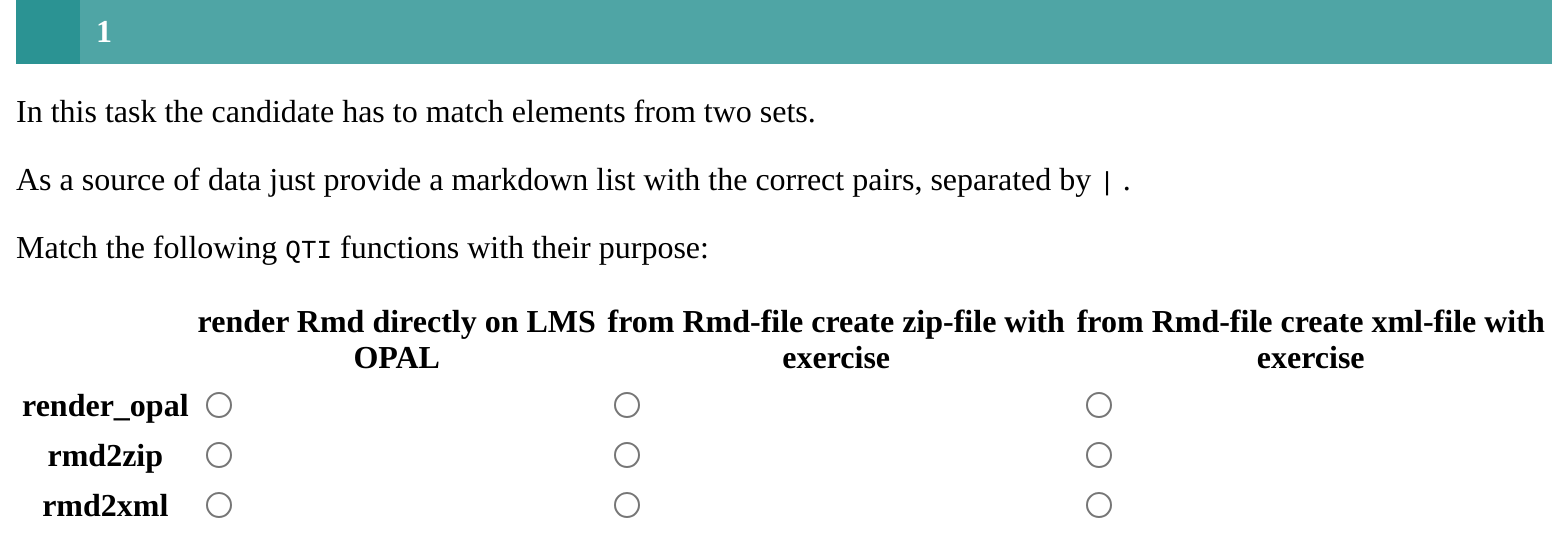
\includegraphics[width=1\textwidth,height=\textheight]{images/directedpair-complex.jpg}
\caption{\label{dp2opal}More complex directed pair task rendered in OPAL}
\end{figure}

\section{YAML attributes}\label{YAML-attributes-6}

\noindent\textbf{type}\label{type-6}

Has to be \texttt{pair} or \texttt{dp}.

\noindent\textbf{identifier}\label{identifier-6}

This is the ID of the task, useful for later data analysis of results. The default is the file name. If you are doing extensive data analysis later on it makes sense to
specify a meaningful identifier. In all other cases, the file name should be
fine.

\noindent\textbf{title}\label{title-6}

Title of the task. Can be displayed to students depending on
the learning management system settings. Default is the file name.

\noindent\textbf{orientation}\label{orientation-2}

Defines the \texttt{vertical} or \texttt{horizontal} mode of displaying responses. Default is \texttt{vertical}.

\noindent\textbf{shuffle}\label{shuffle-3}

If \texttt{true} (the default), randomizes the order of the elements. Only in rare occasions it makes sense to have a strict order of elements (setting shuffle to \texttt{false}).

\noindent\textbf{points}\label{points-7}

How many points are given for the whole task. Default is \(0.5\cdot n\), where \(n\) is the number of pairs.

\noindent\textbf{abbr\_id}\label{abbr_id}

If \texttt{abbr\_id} is not specified, \texttt{rqti} generates the identifiers \texttt{right\_1}, \texttt{right\_2}, \ldots{} \texttt{right\_N} and \texttt{left\_1}, \texttt{left\_2}, \ldots{} \texttt{left\_N}. However, these lack inherent semantics. To enhance clarity, some users might want to use the \texttt{abbr\_id} parameter, which introduces abbreviated identifiers based on the text of the pairs. The utility of these abbreviations varies based on item length, but they consistently offer more meaningful identifiers compared to non-semantic alternatives.

\section{Feedback}\label{feedback-6}

Feedback can be provided with the section

\begin{itemize}
\tightlist
\item
  \textbf{\# feedback} (general feedback, displayed every time, without conditions)
\item
  \textbf{\# feedback+} (only provided if student reaches all points)
\item
  \textbf{\# feedback-} (only provided if student does not reach all points)
\end{itemize}

\section{Some advice on directed pair tasks}\label{some-advice-on-directed-pair-tasks}

Directed pairs are forced choice tasks, so they have similar problems as single choice and multiple choice tasks (guessing). A specific problem of directed pairs is that answers are not independent. Making a mistake will lead to additional mistakes because two elements are blocked by one match. Use directed pairs with care.

One might think that directed pairs are superfluous because match tables serve the same purpose. The difference is that in match tables either the row or column can be used more than once. For directed pairs, matching a pair makes both elements unavailable for further matching. This is unique, so there are use cases for directed pairs. But it is important to note that match tables can also represent a direct pair, meaning both directed pairs and match tables can serve as interfaces to the same concept. However, match tables are generally more flexible and are often the preferred choice (refer to Chapter \ref{table-tasks} \href{table.html}{Table tasks} for more details).

\chapter{Table tasks}\label{table-tasks}

In this type of task, the candidate matches rows with columns in a table. This format is often used when multiple questions need to be displayed concisely. Table tasks are highly versatile and are ideal for creating both single-choice and multiple-choice questions.

\section{Minimum version}\label{minimum-version-7}

A minimum template is automatically created when you initiate an \texttt{rqti} project through RStudio. Alternatively, it can be added by clicking on \texttt{New\ file\ \textrightarrow{}\ R\ Markdown\ \textrightarrow{}\ From\ Template}. The \texttt{rqti} templates end with \texttt{\{rqti\}}. Here we look at the templates \texttt{table\ (simple)} and \texttt{table\ (complex)}.

The minimum you need to provide is the \texttt{type:\ table} in the YAML-section and a table in a section called \textbf{\#question}:

\begin{Shaded}
\begin{Highlighting}
---
type: table
knit: rqti::render_qtijs
---

# question

Specify any kind of table with the table entries representing the number of
points for the response. The table has to be the last element of the question
section!

The `rqti` package is clever enough to transform your table into the appropriate
QTI object (single choice, multiple choice, directed pair). Of course you can
also just load a csv and print it as a markdown table via
`knitr::kable(yourtable)`

Hint: Use visual editing mode in RStudio to quickly change your table.

|      |27|36 |25| 6 |
|------|--|---|--|---|
|4*9 = |0 |0.5|0 | 0 |
|3*9 = |1 |0  |0 | 0 |
|5*5 = |0 |0  |1 | 0 |
|2*3 = |0 |0  |0 | 1 |
|12*3 =|0 |1  |0 | 0 |

# feedback

Provide your feedback here. For tables it is difficult to provide useful
feedback because there are usually many questions. But most learning management
systems will at least show which answers are correct and incorrect.
\end{Highlighting}
\end{Shaded}

Clicking the Knit-Button will produce the output in Figure \ref{tbl1qtijs}.

\begin{figure*}
\centering
\includegraphics[width=1\textwidth,height=\textheight]{images/xml/table-simple.jpg}
\caption{\label{tbl1qtijs}Preview of table task rendered by qtijs}
\end{figure*}

\noindent Alternatively, change the knit parameter to \texttt{knit:\ rqti::render\_opal} (see Chapter \ref{working-with-the-opal-api} \href{api_opal.html}{Working with the OPAL API}) to upload to opal directly, producing the output Figure \ref{tbl1opal}.

\begin{figure}
\centering
\includegraphics[width=1\textwidth,height=\textheight]{images/table-simple.jpg}
\caption{\label{tbl1opal}Preview of table task rendered by OPAL}
\end{figure}

In the Rmd file, table entries indicate the points awarded for each response. Any positive number is considered correct. You can also assign negative numbers, which will reduce the total score, but the overall score will never go below zero. You can specify the number of correct responses per row and column as needed, which typically influences how the table is presented. For example, there are special table configurations where only one row is correct per column, and vice versa. The \texttt{rqti} package handles these cases automatically.

However, it is important to note that if your table represents a directed pair, the \texttt{rqti} package will automatically convert it into a directed pair task. If you prefer to keep it as a standard table, use \texttt{as\_table:\ true} in the YAML section of your Rmd file.

The overall points for the task are calculated as the sum of the positive table entries.

Of course you can also load a csv file (or any other table-like file) and print it as a markdown table via \texttt{knitr::kable(yourtable)}. Just keep in mind that the table has to be the last element of the question section. Styles can be applied to the table and are usually handled well by learning management systems. But keep in mind that style attributes might not be conforming to the QTI standard.

In this example, a feedback section was also included. While feedback is optional, it is generally beneficial to provide some explanation to students. However, offering detailed feedback can be challenging for table tasks, especially when questions are presented in random order. Most learning management systems at least indicate which answers are correct or incorrect, so feedback can be more general, focusing on the overall topic.

\section{More control}\label{more-control-7}

If you want to have more fine-grained control, consider the Rmd template \texttt{table\ (complex)}, which uses more YAML attributes.

\begin{Shaded}
\begin{Highlighting}
---
type: table
knit: rqti::render_qtijs
identifier: TOPIC1_Q001 # think twice about this id for later data analysis!
title: A meaningful title that can be displayed in the LMS
shuffle_cols: false
shuffle_rows: true
abbr_id: true
---

# question

Specify any kind of table with the table entries representing the number of
points for the response. The table has to be the last element of the question
section!

The `rqti` package is clever enough to transform your table into the appropriate
QTI object (single choice or multiple choice). Of course you can also just load
a csv and print it as a markdown table via `knitr::kable(yourtable)`

Use visual editing mode in RStudio to quickly change your table.

|      |27|36 |25| 6 |
|------|--|---|--|---|
|4*9 = |0 |0.5|0 | 0 |
|3*9 = |1 |0  |0 | 0 |
|5*5 = |0 |0  |1 | 0 |
|2*3 = |0 |0  |0 | 1 |
|12*3 =|0 |1  |0 | 0 |


# feedback

Provide your feedback here. For tables it is difficult to provide useful
feedback because there are usually many questions. But most learning management
systems will at least show which answers are correct and incorrect.
\end{Highlighting}
\end{Shaded}

Which, in OPAL, renders as illustrated in Figure \ref{tbl2opal}. You can see that the order of the columns is now the same as in the source table.

\begin{figure}[htb]
\centering
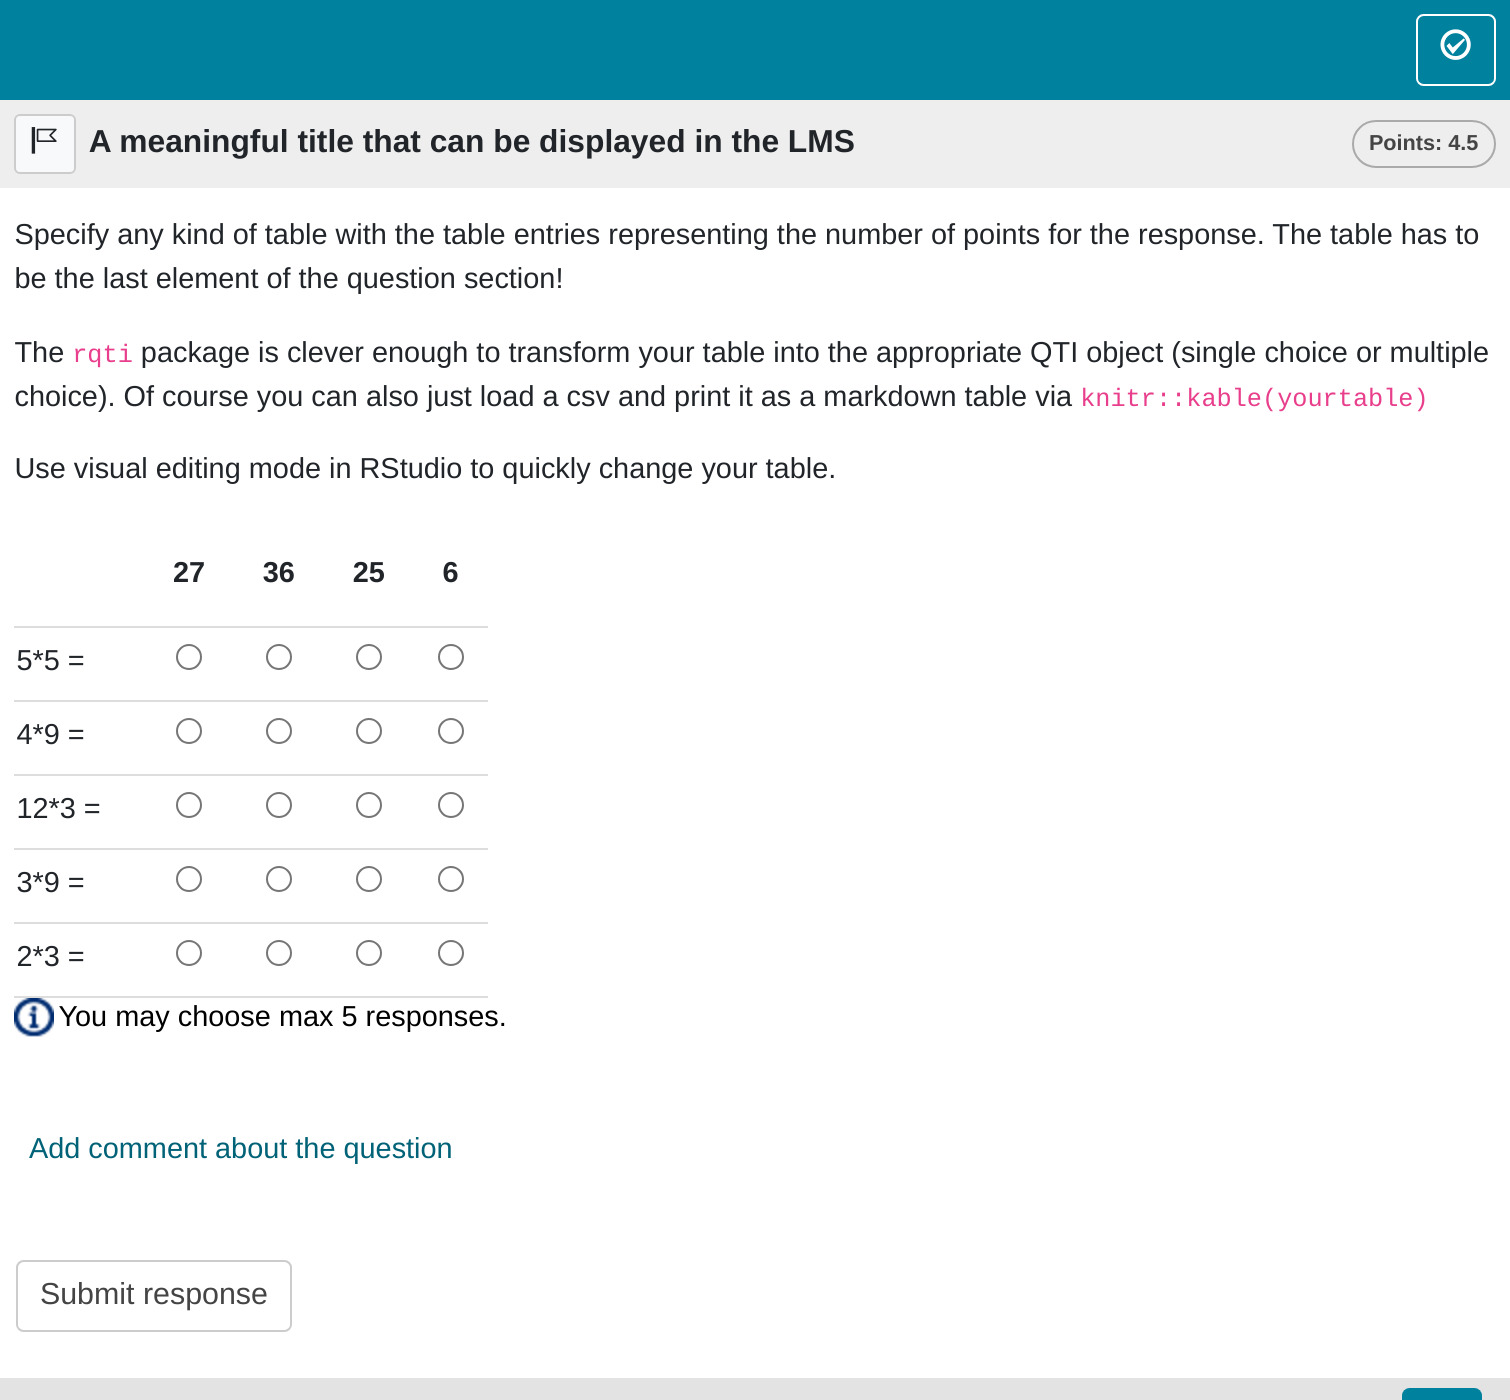
\includegraphics[width=1\textwidth,height=\textheight]{images/table-complex.jpg}
\caption{\label{tbl2opal}Preview of complex table task in the learning management system OPAL}
\end{figure}

\section{YAML attributes}\label{YAML-attributes-7}

\noindent\textbf{type}\label{type-7}

Has to be \texttt{table} or \texttt{match}.

\noindent\textbf{identifier}\label{identifier-7}

This is the ID of the task, useful for later data analysis of results. The default is the file name. If you are doing extensive data analysis later on it makes sense to specify a meaningful identifier. In all other cases, the file name should be
fine.

\noindent\textbf{title}\label{title-7}

Title of the task. Can be displayed to students depending on the learning management system settings. Default is the file name.

\noindent\textbf{shuffle}\label{shuffle-4}

If \texttt{true} (the default), randomizes the order of rows and columns. Only in rare occasions it makes sense to set shuffle to \texttt{false}. For instance, when asking for scale types (nominal, ordinal, interval, ratio) it is better to stick to this order instead of a random one. Overwrites \texttt{shuffle\_rows} and \texttt{shuffle\_cols}.

\noindent\textbf{shuffle\_rows}\label{shuffle_rows}

Only shuffle the rows. Default is \texttt{true}. Overwritten by \texttt{shuffle}.

\noindent\textbf{shuffle\_cols}\label{shuffle_cols}

Only shuffle the columns. Default is \texttt{true}. Overwritten by \texttt{shuffle}.

\noindent\textbf{abbr\_id}\label{abbr_id-1}

Defines the use of an abbreviation as a way to generate row and column identifiers. Explained in more detail in the section \ref{ids} \hyperref[ids]{Managing identifiers}.

\section{Feedback}\label{feedback-7}

Feedback can be provided with the section

\begin{itemize}
\tightlist
\item
  \textbf{\# feedback} (general feedback, displayed every time, without conditions)
\item
  \textbf{\# feedback+} (only provided if student reaches all points)
\item
  \textbf{\# feedback-} (only provided if student does not reach all points)
\end{itemize}

\section{Managing identifiers}\label{ids}

The identifiers for rows and columns are valuable for later data analysis. If you plan to conduct extensive analysis, it is beneficial to assign meaningful and easily recognizable identifiers.

Currently, there are two methods for creating row and column identifiers:

\begin{enumerate}
\def\labelenumi{\arabic{enumi}.}
\tightlist
\item
  \textbf{Default Method}: By default, \texttt{rqti} generates identifiers in the format \texttt{row\_1}, \texttt{row\_2}, \ldots, \texttt{row\_N}, and \texttt{col\_1}, \texttt{col\_2}, \ldots, \texttt{col\_N}.
\item
  \textbf{Abbreviation Method}: By setting \texttt{abbr\_id:\ true} in the YAML section of your Rmd file, \texttt{rqti} generates identifiers by combining the first word of a row or column element with an abbreviation of the remaining text. For example, the element ``Mean Value Theorem for Integrals'' would be shortened to ``Mean\_VTfI''. If a row or column name starts with digits, \texttt{rqti} automatically adds a ``row'' or ``col'' prefix, as identifiers cannot begin with a number. Special characters are also removed.
\end{enumerate}

After experimenting with various approaches, we settled on these straightforward methods. If you require more control over the identifiers, please open an issue on GitHub: \url{https://github.com/shevandrin/rqti/issues}. We are open to reconsidering the available options.

\section{Some advice on table tasks}\label{some-advice-on-table-tasks}

Table tasks are forced choice tasks, so they suffer from the sample problems as \href{singlechoice.html}{single choice} and \href{multiplechoice.html}{multiple choice} tasks. The advantage of table tasks is that they are easy so manage (e.g.~in csv-tables) and many questions can be asked at once, using little space.

\chapter{Adding metadata}\label{adding-metadata}

Metadata---including details about creators, rights, and descriptions---is essential for ensuring accountability, legal compliance, and clarity in the management and use of assessment items and tests. This information helps track content origin and ownership, while also providing clear descriptions that facilitate better organization and retrieval of assessment resources.

We utilize ONYX's metadata implementation, which largely supports the IEEE Learning Object Metadata (LOM) standard. As a result, metadata is stored in XML format within the IMS manifest of the test data. However, it is important to note that this metadata may not be displayed by other learning management systems, and even OPAL may overwrite it. The primary purpose is to maintain metadata within the original xml files being shared.

Here is an example of metadata with two contributors in the YAML section:

\begin{Shaded}
\begin{Highlighting}
---
title: Demonstration of metadata
type: essay
knit: rqti::render_qtijs
identifier: demo_metadata

metadata:
  contributor:
    - name: Andrey Shevandrin
      role: author
    - name: Johannes Titz
      role: author
  description: Demonstration of metadata
  rights: CC BY SA Andrey Shevandrin and Johannes Titz (2024).
---

# question

Essay exercise with metadata attributes in the YAML section.
\end{Highlighting}
\end{Shaded}

Currently, the metadata may contain the following information:

\begin{itemize}
\tightlist
\item
  \textbf{description}: A string providing a description of the task content.
\item
  \textbf{rights}: A string outlining the usage rights and terms associated with the task.
\item
  \textbf{version}: A string indicating the version of the task.
\item
  \textbf{contributor}: A list of contributor details, where each contributor entry may include the following information:

  \begin{itemize}
  \tightlist
  \item
    \textbf{name}: A string representing the contributor's name.
  \item
    \textbf{role}: A string specifying the type of contribution. Possible values include: author, publisher, unknown, initiator, terminator, validator, editor, graphical designer, technical implementer, content provider, technical validator, educational validator, script writer, instructional designer, and subject matter expert. By default, \texttt{rqti} sets this value to ``author''.
  \item
    \textbf{contribution\_date}: A string representing the date of contribution. By default, \texttt{rqti} sets this to the current system date.
  \end{itemize}
\end{itemize}

If you are working on a set of tasks, setting metadata for each one individually can be tedious. To streamline this process, you can use the environment variables \texttt{RQTI\_AUTHOR} and \texttt{RQTI\_RIGHTS}, which will automatically populate these fields with default values.

For example, you can create an \texttt{.Rprofile} file and set the default author and usage rights as follows:

\begin{Shaded}
\begin{Highlighting}[]
\FunctionTok{Sys.setenv}\NormalTok{(}\AttributeTok{RQTI\_AUTHOR =} \StringTok{"Ada Lovelace"}\NormalTok{)}
\FunctionTok{Sys.setenv}\NormalTok{(}\AttributeTok{RQTI\_RIGHTS =} \StringTok{"CC BY SA"}\NormalTok{)}
\end{Highlighting}
\end{Shaded}

If you need to use non-default values, just specify the YAML attributes, which will override the environment variables.

\chapter{Sections and Tests}\label{sections-and-tests}

Creating individual tasks is not particularly useful, as the goal is usually to combine various tasks into a comprehensive test. In the QTI standard, a test consists of one or more sections. Each section can contain a mix of tasks or subsections, offering great flexibility in test structure. Sections can be customized with parameters like time limits and task shuffling. Additionally, tests can include parameters such as time limits, the option to add comments to tasks, supplementary files, or even a calculator---depending on the capabilities of the LMS. %e other features of rqti, sections and tests must be configured using functions rather than within an Rmd file.

The \texttt{rqti} package makes it very simple to mix different sources of task files:

\begin{itemize}
\tightlist
\item
  \textbf{Rmd (md) files}: You can use Rmarkdown files that are consistent with the \texttt{rqti} package (the \texttt{exams} package will not work, but see below)
\item
  \textbf{QTI XML files}: These files should be valid regarding the QTI standard. To use your Rmd-files from the \texttt{exams} package you can convert them to xml first.
\item
  \textbf{Objects of S4 \texttt{rqti} classes}: You can also use objects from the \texttt{rqti} package directly. See Chapter \ref{rqti-oop-model} \href{rqti_oop_model.html}{rqti OOP model}.
\end{itemize}

\section{\texorpdfstring{Using the \texttt{section} and \texttt{test} functions}{Using the section and test functions}}\label{using-the-section-and-test-functions}

Although it is possible to feed a test with tasks directly, we suggest to always use a section, as this provides more flexibility and avoids several problems. Even if you do not need a section, you can just create a root section and put the tasks there.

We designed a simple wrapper for sections. Here we load some files from our package and use the function \texttt{section} to create the section. Note that we request 10 different variants of all tasks.

\begin{Shaded}
\begin{Highlighting}[]
\NormalTok{path }\OtherTok{\textless{}{-}}\NormalTok{ fs}\SpecialCharTok{::}\FunctionTok{path\_package}\NormalTok{(}\StringTok{"exercises"}\NormalTok{, }\AttributeTok{package =} \StringTok{"rqti"}\NormalTok{)}
\NormalTok{files }\OtherTok{\textless{}{-}} \FunctionTok{paste0}\NormalTok{(path, }\StringTok{"/"}\NormalTok{, }\FunctionTok{c}\NormalTok{(}\StringTok{"gap1.Rmd"}\NormalTok{, }\StringTok{"gap2.Rmd"}\NormalTok{))}
\NormalTok{root\_section }\OtherTok{\textless{}{-}} \FunctionTok{section}\NormalTok{(}\AttributeTok{content =}\NormalTok{ files, }\AttributeTok{n\_variants =} \DecValTok{10}\NormalTok{)}
\end{Highlighting}
\end{Shaded}

Now we can make a test out of this and upload it to OPAL. Again there are helpers for that: \texttt{test} and \texttt{test4opal}. \texttt{test} is more general and is always consistent with the QTI model, whereas \texttt{test4opal} can use additional OPAL-specific parameters that are not necessarily consistent with QTI.

\begin{Shaded}
\begin{Highlighting}[]
\NormalTok{test }\OtherTok{\textless{}{-}} \FunctionTok{test}\NormalTok{(root\_section, }\StringTok{"test1"}\NormalTok{)}
\CommentTok{\# createQtiTest is a method of the OOP class \textasciigrave{}test\textasciigrave{}}
\FunctionTok{createQtiTest}\NormalTok{(test, }\AttributeTok{zip\_only =}\NormalTok{ T)}
\NormalTok{repo }\OtherTok{\textless{}{-}} \FunctionTok{upload2opal}\NormalTok{(}\StringTok{"test1.zip"}\NormalTok{, }\AttributeTok{open\_in\_browser =}\NormalTok{ F)}
\end{Highlighting}
\end{Shaded}

Note that you could also call \texttt{upload2opal(test)} directly. We just wanted to demonstrate how to write out a test locally before uploading it somewhere. Of course you can also just use \texttt{render\_qtijs(test)} to preview the test locally--- but in qtijs you will not see the structure of the test, so we use OPAL for demonstration purposes.

We now have 10 variants of the test, two of which are displayed in Figures \ref{a1} and \ref{b1}.

\begin{figure*}
\centering
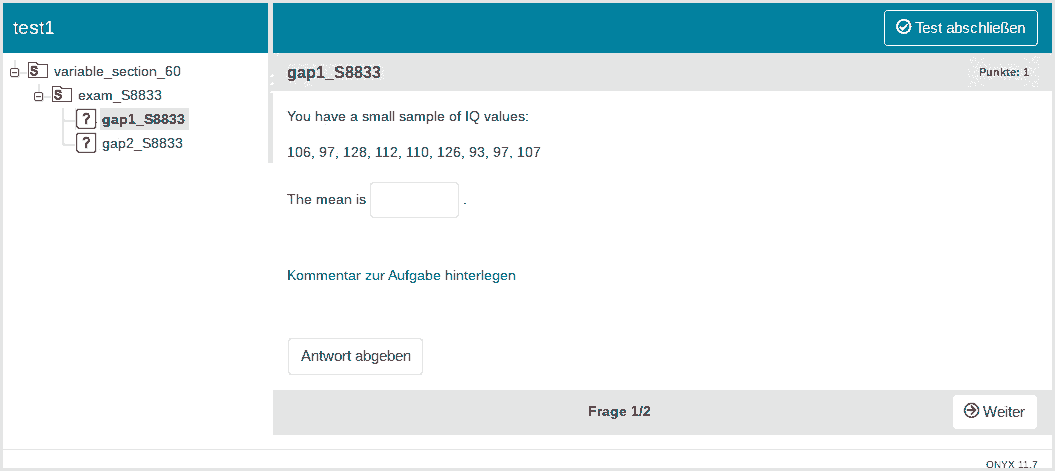
\includegraphics[width=1\textwidth,height=\textheight]{images/Atest1.jpg}
\caption{\label{a1}Test structure for seed 8833.}
\end{figure*}

\begin{figure*}
\centering
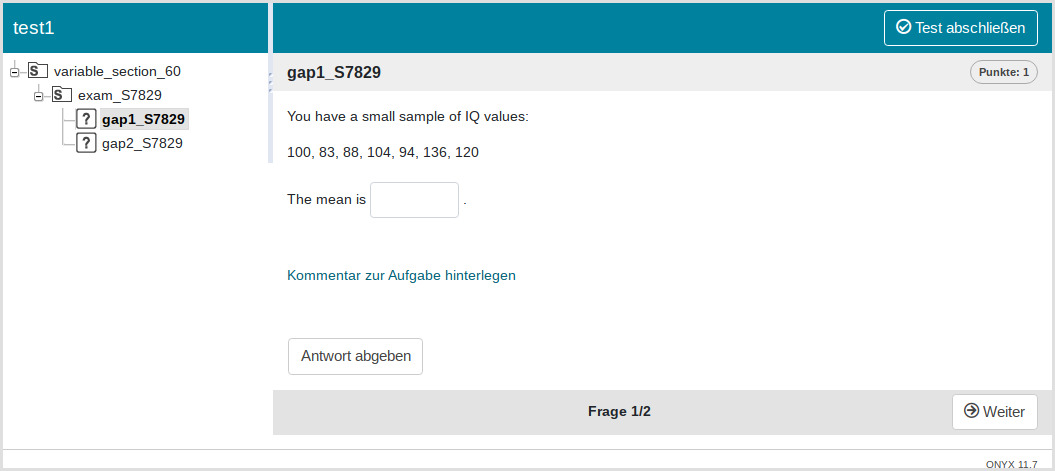
\includegraphics[width=1\textwidth,height=\textheight]{images/Btest1.jpg}
\caption{\label{b1}Test structure for seed 7829.}
\end{figure*}

After the root section you can see the section exam\_8833 (Figure \ref{a1}) and exam\_S7829 (Figure \ref{b1}). There are actually 8 more (10 in total) and if you restart the exam, you will get one randomly assigned. You can try it yourself: \url{https://bildungsportal.sachsen.de/opal/auth/RepositoryEntry/46081048578}. Note that the tasks inside the section have the same seed.

To summarize so far: You can just pass your task files to the \texttt{content} parameter in \texttt{section} and define how many variants you would like to create of each file.

Creating multiple variants is mainly useful for random tasks, like providing different numbers for statistical calculations in gap tasks. On the other hand, single-choice and multiple-choice tasks are usually fixed and can be organized into a separate section, which aids in later data analysis. While each task needs a unique identifier, you generally do not want different identifiers for non-random tasks. To create an additional section, we can call:

\begin{Shaded}
\begin{Highlighting}[]
\NormalTok{non\_random\_tasks }\OtherTok{\textless{}{-}} \FunctionTok{paste0}\NormalTok{(path, }\StringTok{"/"}\NormalTok{, }\FunctionTok{c}\NormalTok{(}\StringTok{"sc1.Rmd"}\NormalTok{, }\StringTok{"mpc1.Rmd"}\NormalTok{))}
\NormalTok{root\_section }\OtherTok{\textless{}{-}} \FunctionTok{list}\NormalTok{(}\FunctionTok{section}\NormalTok{(files, }\AttributeTok{n\_variants =} \DecValTok{10}\NormalTok{),}
                     \FunctionTok{section}\NormalTok{(non\_random\_tasks))}
\end{Highlighting}
\end{Shaded}

Note that we use a list here for the root section. This is important as the \texttt{test} functions expect a list to be more flexible with different inputs (e.g.~objects instead of files). Now we can again make a test out of this and upload it to OPAL:

\begin{Shaded}
\begin{Highlighting}[]
\NormalTok{test }\OtherTok{\textless{}{-}} \FunctionTok{test4opal}\NormalTok{(root\_section, }\StringTok{"test2"}\NormalTok{)}
\FunctionTok{createQtiTest}\NormalTok{(test, }\AttributeTok{zip\_only =}\NormalTok{ T)}
\NormalTok{repo }\OtherTok{\textless{}{-}} \FunctionTok{upload2opal}\NormalTok{(}\StringTok{"test2.zip"}\NormalTok{, }\StringTok{"test2"}\NormalTok{, }\AttributeTok{open\_in\_browser =}\NormalTok{ F)}
\end{Highlighting}
\end{Shaded}

In OPAL this will create the structure displayed in Figures \ref{a2} and \ref{b2}.

\begin{figure*}
\centering
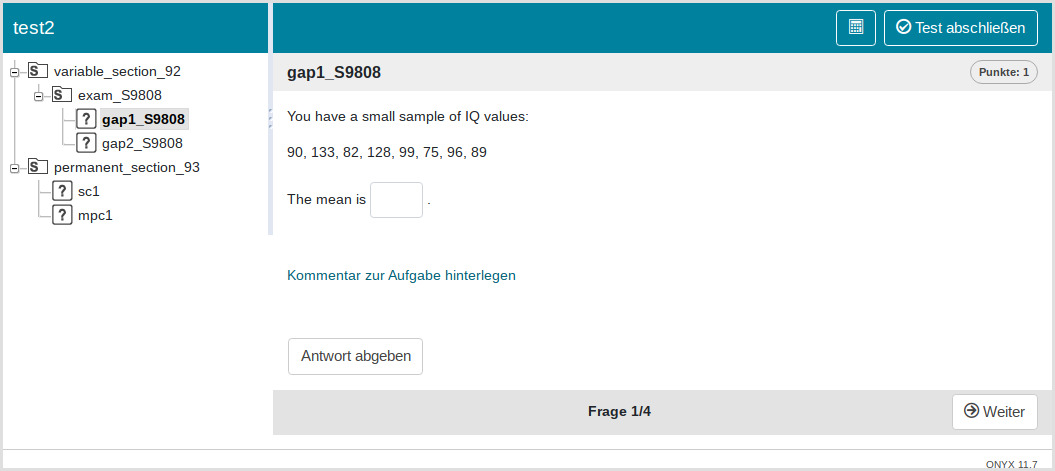
\includegraphics[width=1\textwidth,height=\textheight]{images/Atest2.jpg}
\caption{\label{a2}Test structure with one fixed section, seed 9808.}
\end{figure*}

\begin{figure*}
\centering
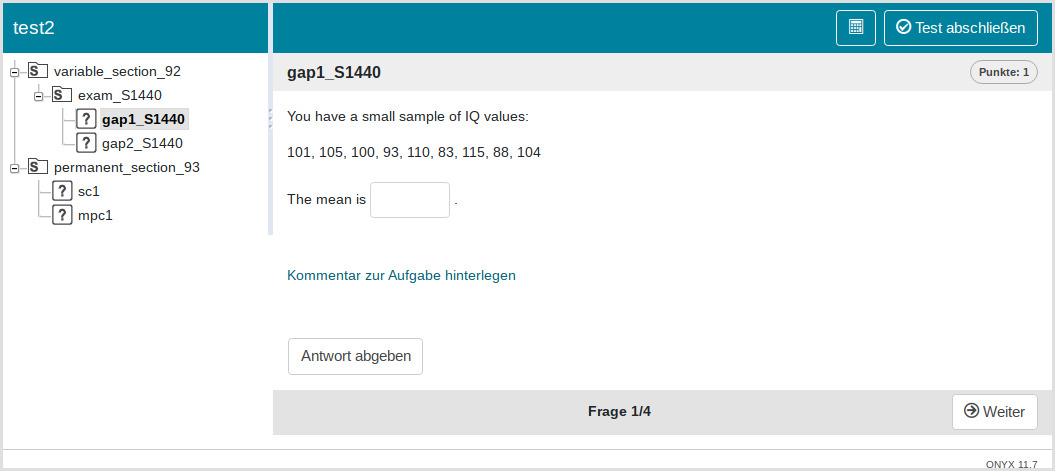
\includegraphics[width=1\textwidth,height=\textheight]{images/Btest2.jpg}
\caption{\label{b2}Test structure with one fixed section, for seed 8833.}
\end{figure*}

As you can see, we still have our variable section with different variants (two of them are displayed in the Figures). But now, we also have a fixed section that is the same for all tests. Try it out yourself: \url{https://bildungsportal.sachsen.de/opal/auth/RepositoryEntry/46075805699}.

Note that the function \texttt{section} returns an \texttt{AssessmentSection} \texttt{rqti}-object:

\begin{Shaded}
\begin{Highlighting}[]
\FunctionTok{lapply}\NormalTok{(root\_section, class)}
\CommentTok{\#\textgreater{} [[1]]}
\CommentTok{\#\textgreater{} [1] "AssessmentSection"}
\CommentTok{\#\textgreater{} attr(,"package")}
\CommentTok{\#\textgreater{} [1] "rqti"}
\CommentTok{\#\textgreater{} }
\CommentTok{\#\textgreater{} [[2]]}
\CommentTok{\#\textgreater{} [1] "AssessmentSection"}
\CommentTok{\#\textgreater{} attr(,"package")}
\CommentTok{\#\textgreater{} [1] "rqti"}
\end{Highlighting}
\end{Shaded}

The entire \texttt{rqti}-package relies on S4 Object-Oriented Programming (OOP), where tasks, sections, and tests are treated as distinct objects. If you are not accustomed to OOP, it might seem unfamiliar at first, but you do not need to delve into all the technical details to use it effectively. Simply utilize the provided helper functions, and you should navigate through with ease.

To customize your sections and tests, check out the references: \texttt{?section} and \texttt{?test} or \texttt{?test4opal}. All parameters are explained there in more detail. We plan to add examples of the most useful parameters to this documentation in the future.

\section{Two approaches for parallel versions of a task}\label{two-approaches-for-parallel-versions-of-a-task}

By default the \texttt{section} function creates different variants of a task by drawing different seeds and creating subsections with these seeds. There is also a different approach to introduce randomness. Have a look at Figure \ref{scheme}.

\begin{figure*}
\centering
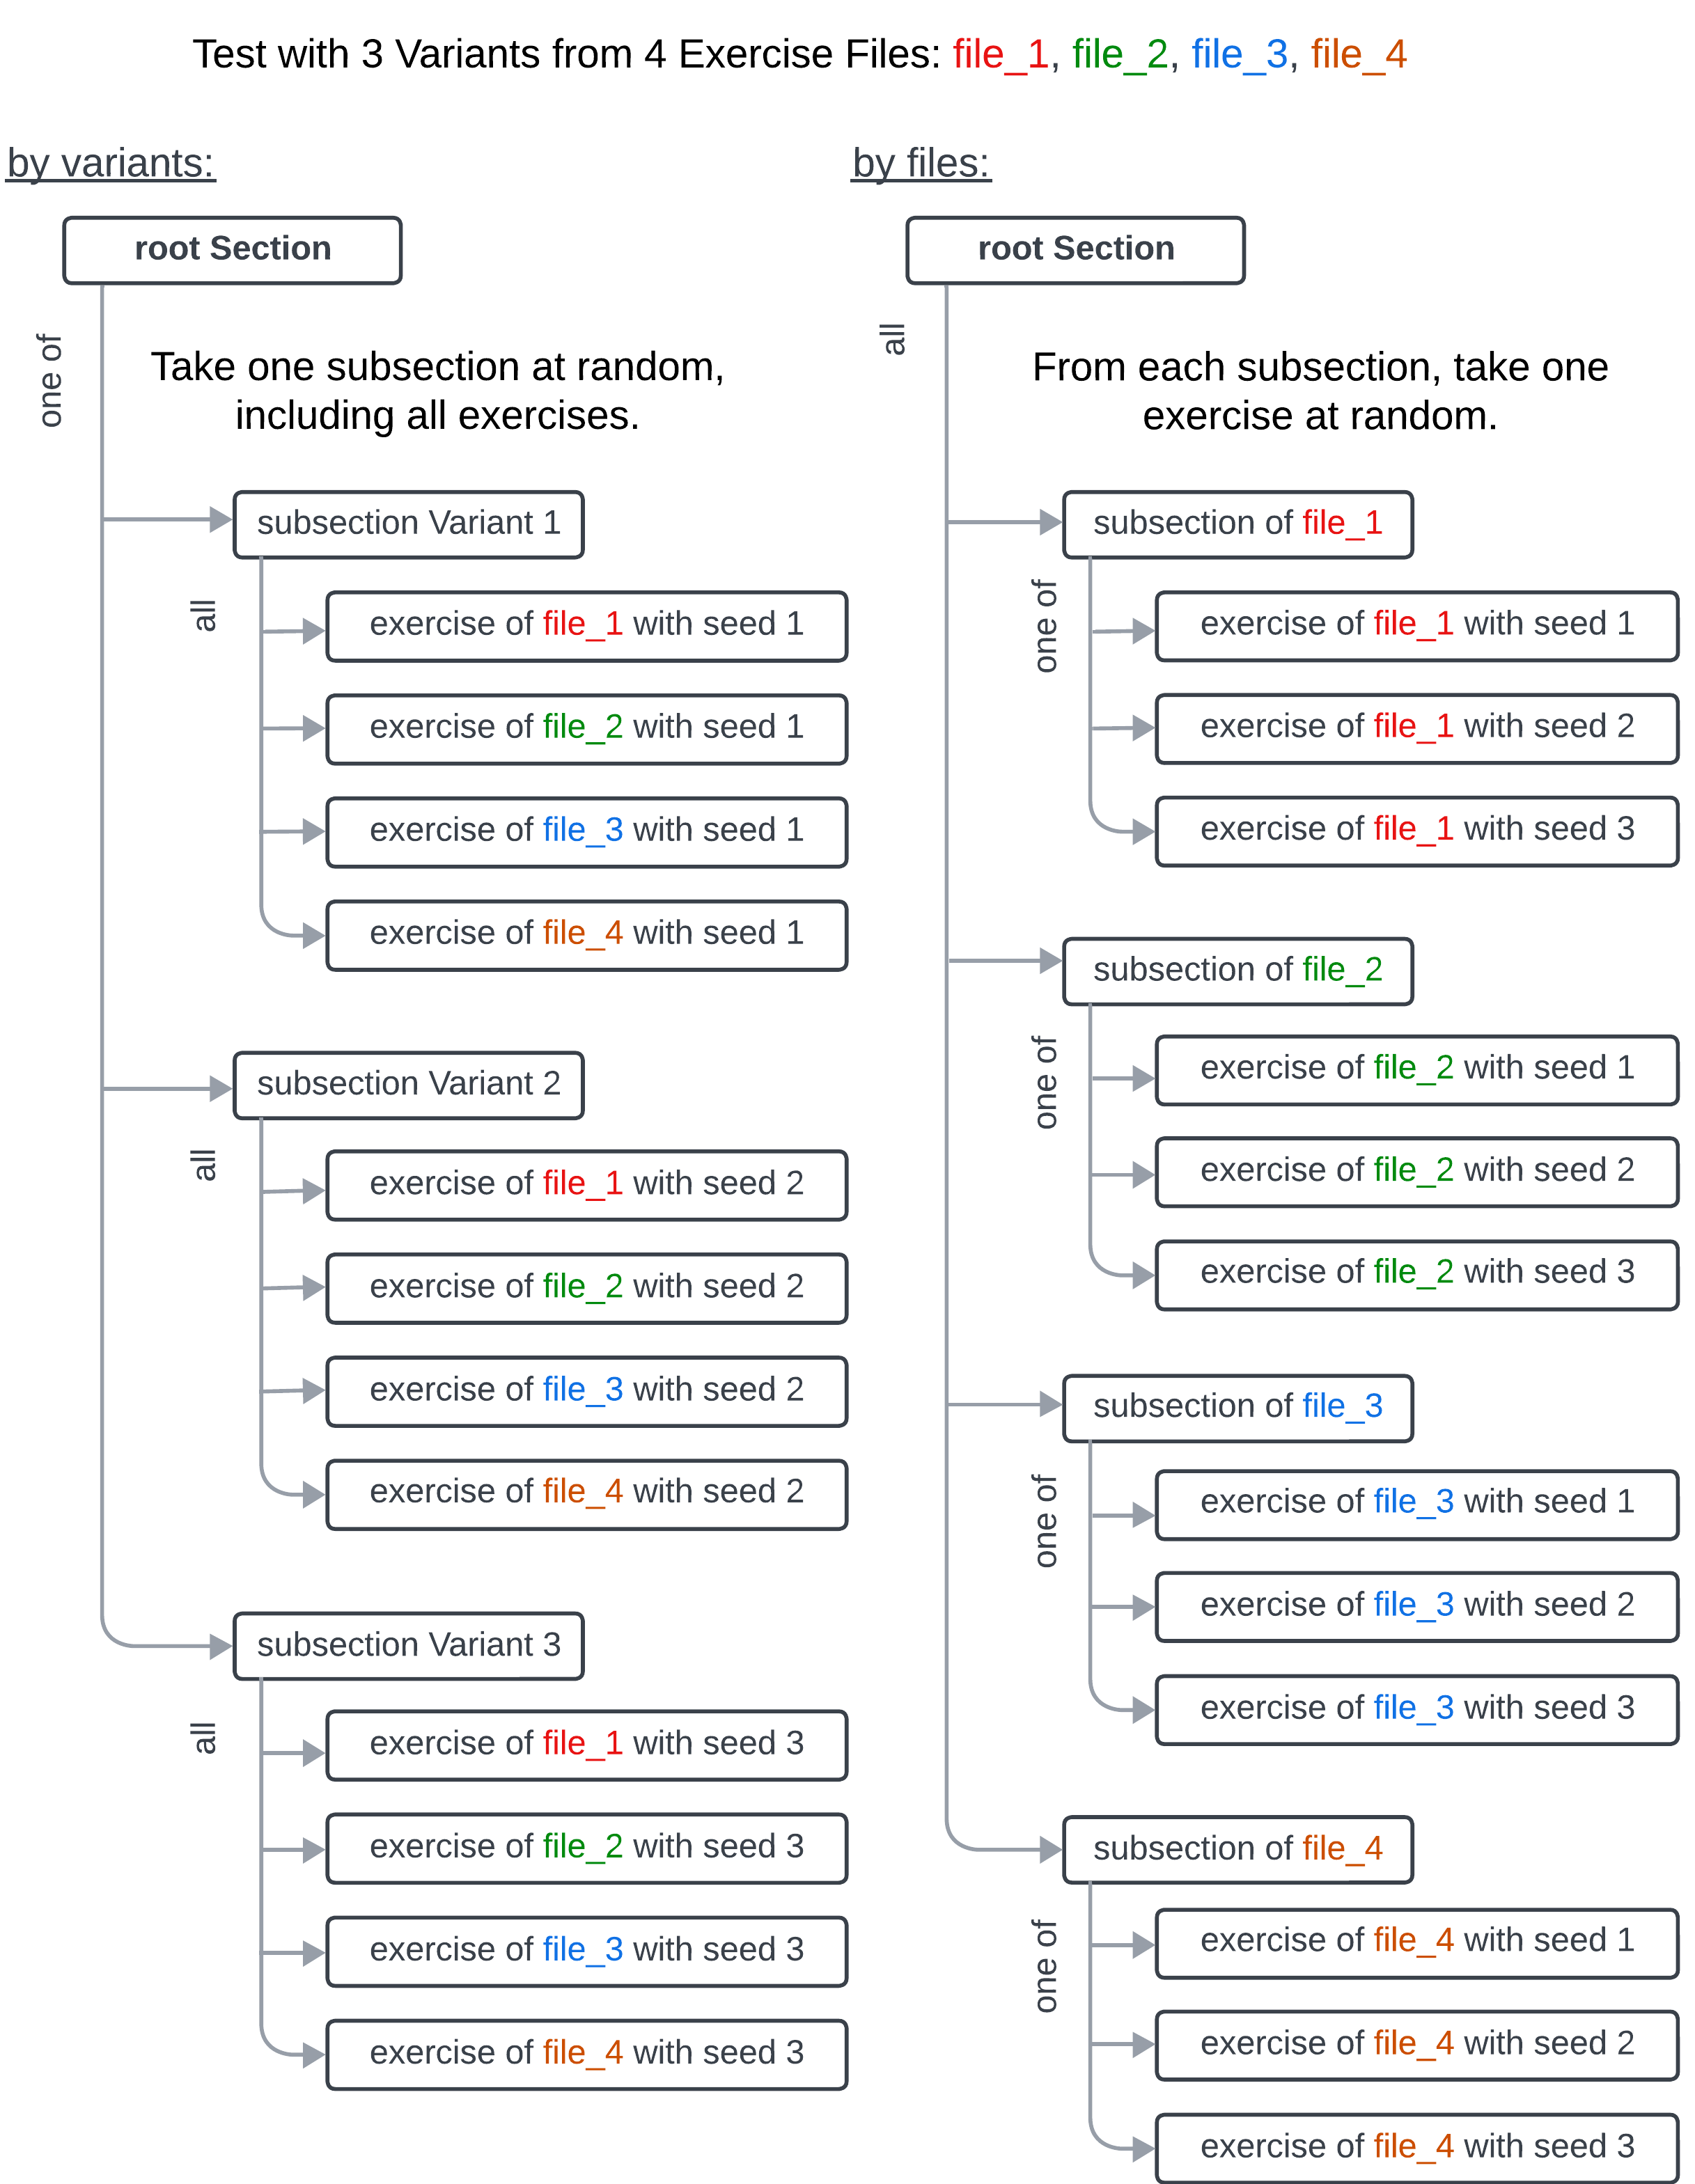
\includegraphics[width=1\textwidth,height=\textheight]{images/sectionsscheme.png}
\caption{\label{scheme}Two approaches for structuring parallel versions of tasks}
\end{figure*}

On the left-hand side, three distinct subsections were generated, each housing the same task files but with \textbf{different variants}. A participant, starting at the root section, is randomly assigned to one of these subsections, encountering all tasks within that specific subsection. This setup is generally satisfactory for most instructors conducting exams. It ensures that all participants within a subsection encounter the same set of tasks, facilitating psychometric analysis. However, a drawback is the potential for forbidden collaboration between participants within the same subsection.

On the right-hand side, an alternative strategy was implemented. Each task \textbf{file} now has its dedicated subsection, encompassing its diverse variants. Participants navigate through each section, being assigned only one variant of the task per section. The noteworthy distinction from the other approach lies in the plethora of potential paths available in the test. Given the presence of 3 variants for each of the 4 files, a total of \(3^4 = 81\) paths emerges. While this configuration may complicate psychometric analysis and introduce challenges in maintaining task difficulty equilibrium, it provides a notable advantage in thwarting cheating, as the paths of two students are likely to differ.

However, exercising caution is imperative when adopting this approach, particularly in an exam setting. Interestingly, this setup finds greater utility when exchanging specific tasks among instructors. For instance, generating 20 variants of a task and bundling them into a test allows for easy import as a subtest in other instructors' exams. Notably, such flexibility would not be feasible with the structure on the left-hand side.

To choose between these two versions you can use the parameter \texttt{by} in the sense of \texttt{section} by \texttt{variants} or \texttt{section} by \texttt{files}.

\begin{Shaded}
\begin{Highlighting}[]
\NormalTok{root\_section }\OtherTok{=} \FunctionTok{section}\NormalTok{(}\AttributeTok{content =}\NormalTok{ files, }\AttributeTok{n\_variants =} \DecValTok{3}\NormalTok{, }\AttributeTok{by =} \StringTok{"files"}\NormalTok{)}
\end{Highlighting}
\end{Shaded}

\begin{enumerate}
\def\labelenumi{\arabic{enumi}.}
\tightlist
\item
  For ``by variants'' (left scheme on the picture) use \texttt{by\ =\ "variants"}
\item
  For ``by files'' (right scheme) use \texttt{by\ =\ "files"}
\end{enumerate}

We are still looking for better semantics of these cases, so if you have a good idea, open an issue on our github page: \url{https://github.com/shevandrin/rqti}

\chapter{Working with the OPAL API}\label{working-with-the-opal-api}

The \texttt{rqti} package facilitates seamless content uploads to the OPAL learning management system through its \texttt{upload2opal} function, leveraging the OPAL API. In addition, there are useful functions to get a list of resources and exchanging existing resources in courses.

\section{Prerequisites}\label{prerequisites}

To leverage the functionality of the OPAL API, it is essential for OPAL users to possess the requisite permissions. Access to the system necessitates logging in with a username and password. Utilizing the API through Shibboleth authorization is not supported.

If you currently lack a password-based login, kindly submit a request for one through your IT department. For users affiliated with \textbf{TU Chemnitz}, you can expedite this process by sending an email to \href{mailto:e-learning@tu-chemnitz.de}{\nolinkurl{e-learning@tu-chemnitz.de}}. In your email, explicitly state your need for a password-based login to facilitate API usage, and include your username for reference. You should also state the purpose of API usage. Please be aware that students typically do not possess author rights by default and are required to request such privileges before utilizing the API. To facilitate this process, it is advisable to reach out to your IT and/or OPAL provider for assistance.

To store the username and password, \texttt{rqti} uses the keyring system credential storage. The first time authentication is attempted, it asks for a username and a password and saves them in a key with service name ``rqtiopal''. Once the key is created, it is automatically used in further sessions. It is not recommended to create additional keys unless you have a more complex setup (e.g.~using multiple learning management systems).

Some universities only allow to use the OPAL API in the network of the university. Before calling \texttt{upload2opal()} set up a VPN client accordingly.
For TU Chemnitz see the instructions here: \url{https://www.tu-chemnitz.de/urz/network/access/vpn.html}

\section{Uploading tasks and tests to OPAL}\label{uploading-tasks-and-tests-to-opal}

You can either set the \texttt{knit:\ rqti::render\_opal} parameter in the YAML-section of your Rmd file or just call \texttt{upload2opal()} with the file as the first parameter:

\begin{Shaded}
\begin{Highlighting}[]
\NormalTok{file }\OtherTok{\textless{}{-}} \StringTok{"my\_zip\_file.zip"} \CommentTok{\# or "task.Rmd" or "task.xml"}
\NormalTok{result }\OtherTok{\textless{}{-}} \FunctionTok{upload2opal}\NormalTok{(file)}
\end{Highlighting}
\end{Shaded}

Note that \texttt{rqti}-Rmd files as well as QTI compliant zip archives and xml files are supported.

If you set up OPAL correctly you can expect the following outcome after running the above command:

\begin{enumerate}
\def\labelenumi{\arabic{enumi}.}
\tightlist
\item
  A web browser will open automatically, displaying the OPAL page with your uploaded test or task.
\item
  In your R console, you will receive a status code 200. This status code indicates that the request to upload the content to OPAL was successful.
\item
  The result variable will contain a list with the following data:

  \begin{itemize}
  \tightlist
  \item
    \$key: An identifier for this resource on OPAL, which you can use for reference.
  \item
    \$display\_name: The title of the resource as it appears in the browser on OPAL.
  \item
    \$url: A permanent link to access this resource on OPAL.
  \end{itemize}
\end{enumerate}

\texttt{upload2opal()} always checks the uniqueness of the \texttt{display\_name} in your personal repository of resources on OPAL. If a resource with the same name is found, \texttt{rqti} will overwrite it by default. This is useful for incrementally improving and previewing/testing the task. It avoids cluttering your OPAL repo with dozens of versions of the same task. If there are several resources with the same name, \texttt{upload2opal} will ask you what to do.

By default \texttt{upload2opal()} uses the file name as the \texttt{display\_name}. But you can define your own as the second parameter:

\begin{Shaded}
\begin{Highlighting}[]
\NormalTok{result }\OtherTok{\textless{}{-}} \FunctionTok{upload2opal}\NormalTok{(file, }\AttributeTok{display\_name =} \StringTok{"Exam123"}\NormalTok{)}
\end{Highlighting}
\end{Shaded}

Currently, there is no option to delete tasks via the API. But you can display the URL of a task via:

\begin{Shaded}
\begin{Highlighting}[]
\FunctionTok{get\_resource\_url}\NormalTok{(}\AttributeTok{display\_name =} \StringTok{"Exam123"}\NormalTok{)}
\end{Highlighting}
\end{Shaded}

Or return all resources as a dataframe via:

\begin{Shaded}
\begin{Highlighting}[]
\FunctionTok{get\_resources}\NormalTok{()}
\end{Highlighting}
\end{Shaded}

If you want to have more fine-grained control for uploading, check out the documentation \texttt{?upload2opal}.

\section{Access rights}\label{access-rights}

Note that the access rights of the resource are set to public by default. This might appear unusual, but for creating tasks incrementally this is the best option. If you use any other access rights, you need to login to OPAL via your browser to see the web page, which will log you out via the API. Currently, there is not better solution for this procedure. Take this into account if you upload sensitive content! For instance, tasks that will be used in an upcoming exam. You can set the access rights via

\begin{Shaded}
\begin{Highlighting}[]
\FunctionTok{uplod2opal}\NormalTok{(..., }\AttributeTok{access =}\NormalTok{ ?)}
\end{Highlighting}
\end{Shaded}

\begin{itemize}
\tightlist
\item
  1: only the persons responsible for this learning resource
\item
  2: responsible and other authors
\item
  3: all registered users
\item
  4: public, default value
\end{itemize}

\section{Endpoint}\label{endpoint}

We are using the OPAL instance \textbf{E-Learning-Informationsportal für Sächsische Hochschulen}, so our package sets the endpoint for \texttt{upload2opal} to \emph{\url{https://bildungsportal.sachsen.de/opal/}}. If you use a different OPAL instance, you can either pass this to the \texttt{endpoint} parameter of \texttt{upload2opal} or just set it in .Rprofile: \texttt{Sys.setenv(RQTI\_API\_ENDPOINT\ =\ "yoururl")}. When initiating an \texttt{rqti} project in RStudio through \emph{New Project}, you have the option to configure the API endpoint at that stage. This configuration is also just written to the .Rprofile file.

\section{Error Handling}\label{error-handling}

The most common issues with the API include:

\textbf{403} - Authorization failed. Some universities allow the use of the API only within the university network. You may need to run a VPN client to use the API.
%For TU Chemnitz see here: \url{https://www.tu-chemnitz.de/urz/network/access/vpn.html}
If you already run a VPN client, please check with your IT and/or OPAL provider, whether the API can be used and what configuration you need.

\textbf{401} - Unauthorized. Your RQTI\_API\_USER or RQTI\_API\_PASSWORD are wrong or your credentials are not sufficient to work with the API. Please be aware that students typically do not possess author rights by default and are required to request such privileges before utilizing the API. To facilitate this process, it is advisable to reach out to your IT and/or OPAL provider for assistance.

\section{OPAL specific YAML attributes}\label{opal-specific-YAML-attributes}

There are several opal-specific YAML attributes, which are explicitly explained in Chapters on the task types. Two of them apply on the test level:

\noindent\textbf{calculator}\label{calculator-1}

If a calculator is required for this task, you need to assign the `calculator' attribute the type `simple' or `scientific'.

\noindent\textbf{files}\label{files-1}

If additional files are required to complete this task, you need to assign the `files' attribute a single file path or a list of paths to these files.

Note that setting these two attributes in the Rmd file directly is mainly useful if you work on a single task. For collections of tasks (tests) it is better to set these attributes when creating the test intead of in the Rmd-file.

\chapter{rqti OOP model}\label{rqti-oop-model}

The Rmd interface of \texttt{rqti} is excellent for quickly getting started, but it has some drawbacks. First, it can be quite slow, as the Rmd file must be converted to HTML before it can be used. This delay is especially noticeable when generating several versions of multiple tasks. Additionally, Rmd lacks flexibility in handling task parameters. For instance, while it is possible to select specific questions within a task by passing parameters during knitting, this approach is not very convenient.

Another challenge with Rmd is storing and distributing the files, as there is no standard method for doing so. While you can host the files somewhere, there is no easy way for instructors to know when a new version is available. Ultimately, while Rmd is great for readability, it is not designed for rigorous programming. If you want to fully leverage a programming language when creating exercises and exams, a programming interface is a better choice.

The \texttt{rqti} package offers such an interface, as it uses S4 object-oriented programming (OOP) under the hood. This allows you to create all task types as objects, providing greater flexibility and faster performance. You can also share your tasks by creating an R package. If you are content with Rmd, there is nothing wrong with continuing to use it. However, if you are looking to take your work to the next level, consider creating task objects directly.

First, check out the overview of our classes:

The \texttt{rqti} class model consists of classes that represent types of tasks:

\begin{itemize}
\tightlist
\item
  \texttt{?SingleChoice}
\item
  \texttt{?MultipleChoice}
\item
  \texttt{?Essay}
\item
  \texttt{?Entry}
\item
  \texttt{?Ordering}
\item
  \texttt{?DirectedPair}
\item
  \texttt{?MultipleChoiceTable}
\item
  \texttt{?OneInRowTable}
\item
  \texttt{?OneInColTable}
\end{itemize}

In addition there are classes for the interaction elements of tasks:

\begin{itemize}
\tightlist
\item
  \texttt{?TextGap}
\item
  \texttt{?NumericGap}
\item
  \texttt{?InlineChoice}
\item
  \texttt{?TextGapOpal}
\item
  \texttt{?ModalFeedback}
\item
  \texttt{?CorrectFeedback}
\item
  \texttt{?WrongFeedback}
\end{itemize}

Finally, there are classes for tests and their sections:

\begin{itemize}
\tightlist
\item
  \texttt{?AssessmentSection}
\item
  \texttt{?AssessmentTest}
\item
  \texttt{?AssessmentTestOpal}
\end{itemize}

%\section{Creating objects}\label{creating-objects}

There are two ways to create objects:

\begin{enumerate}
\def\labelenumi{\arabic{enumi}.}
\tightlist
\item
  A call to \texttt{new} with the corresponding class and parameters.
\item
  Using constructor functions (recommended).
\end{enumerate}

Constructor functions share the same names as their corresponding classes, with the first letter in lowercase. These constructors are again categorized into tasks, interactions, and sections/tests.

The following functions create classes representing different types of tasks:

\begin{itemize}
\tightlist
\item
  \texttt{?singleChoice}
\item
  \texttt{?multipleChoice}
\item
  \texttt{?essay}
\item
  \texttt{?entry}
\item
  \texttt{?ordering}
\item
  \texttt{?directedPair}
\item
  \texttt{?multipleChoiceTable}
\item
  \texttt{?OneInRowTable}
\item
  \texttt{?oneInColTable}
\end{itemize}

The following functions create classes representing interactions within tasks:

\begin{itemize}
\tightlist
\item
  \texttt{?textGap}
\item
  \texttt{?numericGap}
\item
  \texttt{?textGapOpal}
\item
  \texttt{?modalFeedback}
\item
  \texttt{?correctFeedback}
\item
  \texttt{?wrongFeedback}
\end{itemize}

The following functions create classes representing tests and their sections:

\begin{itemize}
\tightlist
\item
  \texttt{?assessmentSection}
\item
  \texttt{?assessmentTest}
\item
  \texttt{?assessmentTestOpal}
\end{itemize}

\section{Creating tasks}\label{creating-tasks}

First, it is important to know that you can create an object directly from Rmd files:

\begin{Shaded}
\begin{Highlighting}[]
\NormalTok{scpath }\OtherTok{\textless{}{-}}\NormalTok{ fs}\SpecialCharTok{::}\FunctionTok{path\_package}\NormalTok{(}\StringTok{"rmarkdown/templates/singlechoice{-}simple/skeleton"}\NormalTok{, }
                           \StringTok{"skeleton.Rmd"}\NormalTok{, }\AttributeTok{package =} \StringTok{"rqti"}\NormalTok{)}
\NormalTok{sc }\OtherTok{\textless{}{-}}\NormalTok{ rqti}\SpecialCharTok{:::}\FunctionTok{create\_question\_object}\NormalTok{(scpath)}
\NormalTok{sc}
\CommentTok{\#\textgreater{} An object of class "SingleChoice"}
\CommentTok{\#\textgreater{} Slot "solution":}
\CommentTok{\#\textgreater{} [1] 1}
\CommentTok{\#\textgreater{} }
\CommentTok{\#\textgreater{} Slot "choices":}
\CommentTok{\#\textgreater{} [1] "There is a 5\% probability that you will mistakenly reject the null hypothesis,}
\CommentTok{when it is actually correct. "}
\CommentTok{\#\textgreater{} [2] "There is a 5\% probability that the null hypothesis is correct."                                              }
\CommentTok{\#\textgreater{} [3] "There is a 5\% probability that you will mistakenly reject the alternative}
\CommentTok{hypothesis, when it is correct."   }
\CommentTok{\#\textgreater{} [4] "The test power is 95\%."                                                                                      }
\CommentTok{\#\textgreater{} }
\CommentTok{\#\textgreater{} Slot "choice\_identifiers":}
\CommentTok{\#\textgreater{} [1] "ChoiceA" "ChoiceB" "ChoiceC" "ChoiceD"}
\CommentTok{\#\textgreater{} }
\CommentTok{\#\textgreater{} Slot "shuffle":}
\CommentTok{\#\textgreater{} [1] TRUE}
\CommentTok{\#\textgreater{} }
\CommentTok{\#\textgreater{} Slot "orientation":}
\CommentTok{\#\textgreater{} [1] "vertical"}
\CommentTok{\#\textgreater{} }
\CommentTok{\#\textgreater{} Slot "identifier":}
\CommentTok{\#\textgreater{} [1] "skeleton"}
\CommentTok{\#\textgreater{} }
\CommentTok{\#\textgreater{} Slot "title":}
\CommentTok{\#\textgreater{} [1] "skeleton"}
\CommentTok{\#\textgreater{} }
\CommentTok{\#\textgreater{} Slot "content":}
\CommentTok{\#\textgreater{} [[1]]}
\CommentTok{\#\textgreater{} [1] "\textless{}p\textgreater{}An alpha error of 5\% means that:\textless{}/p\textgreater{}"}
\CommentTok{\#\textgreater{} }
\CommentTok{\#\textgreater{} }
\CommentTok{\#\textgreater{} Slot "prompt":}
\CommentTok{\#\textgreater{} [1] ""}
\CommentTok{\#\textgreater{} }
\CommentTok{\#\textgreater{} Slot "points":}
\CommentTok{\#\textgreater{} [1] 1}
\CommentTok{\#\textgreater{} }
\CommentTok{\#\textgreater{} Slot "feedback":}
\CommentTok{\#\textgreater{} [[1]]}
\CommentTok{\#\textgreater{} An object of class "ModalFeedback"}
\CommentTok{\#\textgreater{} Slot "outcome\_identifier":}
\CommentTok{\#\textgreater{} [1] "FEEDBACKMODAL"}
\CommentTok{\#\textgreater{} }
\CommentTok{\#\textgreater{} Slot "show":}
\CommentTok{\#\textgreater{} [1] TRUE}
\CommentTok{\#\textgreater{} }
\CommentTok{\#\textgreater{} Slot "identifier":}
\CommentTok{\#\textgreater{} [1] "modal\_feedback"}
\CommentTok{\#\textgreater{} }
\CommentTok{\#\textgreater{} Slot "title":}
\CommentTok{\#\textgreater{} character(0)}
\CommentTok{\#\textgreater{} }
\CommentTok{\#\textgreater{} Slot "content":}
\CommentTok{\#\textgreater{} [[1]]}
\CommentTok{\#\textgreater{} [1] "\textless{}p\textgreater{}The correct interpretation is:\textless{}/p\textgreater{}"}
\CommentTok{\#\textgreater{} }
\CommentTok{\#\textgreater{} [[2]]}
\CommentTok{\#\textgreater{} [1] "\textless{}p\textgreater{}There is a 5\% probability that you will mistakenly reject the null}
\CommentTok{hypothesis, when it is correct.\textless{}/p\textgreater{}"}
\CommentTok{\#\textgreater{} }
\CommentTok{\#\textgreater{} [[3]]}
\CommentTok{\#\textgreater{} [1] "\textless{}p\textgreater{}This is based on the typical understanding of a 5\% significance level}
\CommentTok{in hypothesis testing, which means that you are willing to accept a 5\% chance of}
\CommentTok{making a Type I error.\textless{}/p\textgreater{}"}
\CommentTok{\#\textgreater{} }
\CommentTok{\#\textgreater{} }
\CommentTok{\#\textgreater{} }
\CommentTok{\#\textgreater{} }
\CommentTok{\#\textgreater{} Slot "files":}
\CommentTok{\#\textgreater{} character(0)}
\CommentTok{\#\textgreater{} }
\CommentTok{\#\textgreater{} Slot "calculator":}
\CommentTok{\#\textgreater{} character(0)}
\CommentTok{\#\textgreater{} }
\CommentTok{\#\textgreater{} Slot "metadata":}
\CommentTok{\#\textgreater{} An object of class "QtiMetadata"}
\CommentTok{\#\textgreater{} Slot "contributor":}
\CommentTok{\#\textgreater{} [[1]]}
\CommentTok{\#\textgreater{} An object of class "QtiContributor"}
\CommentTok{\#\textgreater{} Slot "name":}
\CommentTok{\#\textgreater{} [1] "Johannes Titz"}
\CommentTok{\#\textgreater{} }
\CommentTok{\#\textgreater{} Slot "role":}
\CommentTok{\#\textgreater{} [1] "author"}
\CommentTok{\#\textgreater{} }
\CommentTok{\#\textgreater{} Slot "contribution\_date":}
\CommentTok{\#\textgreater{} [1] "2024{-}09{-}06"}
\CommentTok{\#\textgreater{} }
\CommentTok{\#\textgreater{} }
\CommentTok{\#\textgreater{} }
\CommentTok{\#\textgreater{} Slot "description":}
\CommentTok{\#\textgreater{} [1] ""}
\CommentTok{\#\textgreater{} }
\CommentTok{\#\textgreater{} Slot "rights":}
\CommentTok{\#\textgreater{} [1] "CC{-}BY{-}NC{-}SA 4.0 https://creativecommons.org/licenses/by{-}nc{-}sa/4.0/"}
\CommentTok{\#\textgreater{} }
\CommentTok{\#\textgreater{} Slot "version":}
\CommentTok{\#\textgreater{} character(0)}
\end{Highlighting}
\end{Shaded}

The structure of the object may seem intimidating at first, but it is largely self-explanatory. For example, it includes a slot named \texttt{solution} for the correct answer and another named \texttt{choices} for the possible options. Additionally, other slots contain objects such as feedback or metadata, which are themselves composed of various slots. While the nested structure can appear complex, each element is logically organized to support the overall functionality.

Now you can render this object with \texttt{render\_qtijs}:

\begin{Shaded}
\begin{Highlighting}[]
\FunctionTok{render\_qtijs}\NormalTok{(sc)}
\end{Highlighting}
\end{Shaded}

You will notice that this approach is much faster than knitting, as it eliminates intermediate steps. The XML file is generated directly from the object representation and then copied to the qtijs server. No need for Pandoc or any other translation tools.

But how would you create this object from scratch? This is not very hard:

\begin{Shaded}
\begin{Highlighting}[]
\NormalTok{choices }\OtherTok{\textless{}{-}} \FunctionTok{c}\NormalTok{(}
  \StringTok{"There is a 5\% probability that you will mistakenly reject the null}
\StringTok{ hypothesis, when it is actually correct."}\NormalTok{,}
  \StringTok{"There is a 5\% probability that the null hypothesis is correct."}\NormalTok{,}
  \StringTok{"There is a 5\% probability that you will mistakenly reject the alternative}
\StringTok{ hypothesis, when it is correct."}\NormalTok{,}
  \StringTok{"The test power is 95\%."}
\NormalTok{)}

\NormalTok{sc2 }\OtherTok{\textless{}{-}} \FunctionTok{singleChoice}\NormalTok{(}\AttributeTok{choices =}\NormalTok{ choices, }
                    \AttributeTok{content =} \FunctionTok{list}\NormalTok{(}\StringTok{"An alpha error of 5\% means that:"}\NormalTok{))}
\end{Highlighting}
\end{Shaded}

Note that the content parameter is a list because it can also contain non-strings. If you use a text string, \texttt{rqti} will give you an error. In the future we will simplify this case. Again, you can render the object:

\begin{Shaded}
\begin{Highlighting}[]
\FunctionTok{render\_qtijs}\NormalTok{(sc2)}
\end{Highlighting}
\end{Shaded}

It looks the same because it is almost the same:

\begin{Shaded}
\begin{Highlighting}[]
\FunctionTok{all.equal}\NormalTok{(sc, sc2)}
\CommentTok{\#\textgreater{} [1] "Attributes: \textless{} Component \textbackslash{}"calculator\textbackslash{}":}
\CommentTok{ Lengths (0, 1) differ (string compare on first 0) \textgreater{}"}
\CommentTok{\#\textgreater{} [2] "Attributes: \textless{} Component \textbackslash{}"choices\textbackslash{}": 2 string mismatches \textgreater{}"                                 }
\CommentTok{\#\textgreater{} [3] "Attributes: \textless{} Component \textbackslash{}"content\textbackslash{}":}
\CommentTok{ Component 1: 1 string mismatch \textgreater{}"                      }
\CommentTok{\#\textgreater{} [4] "Attributes: \textless{} Component \textbackslash{}"feedback\textbackslash{}":}
\CommentTok{ Length mismatch: comparison on first 0 components \textgreater{}"  }
\CommentTok{\#\textgreater{} [5] "Attributes: \textless{} Component \textbackslash{}"files\textbackslash{}":}
\CommentTok{ Lengths (0, 1) differ (string compare on first 0) \textgreater{}"     }
\CommentTok{\#\textgreater{} [6] "Attributes: \textless{} Component \textbackslash{}"identifier\textbackslash{}":} \CommentTok{ 1 string mismatch \textgreater{}"                                }
\CommentTok{\#\textgreater{} [7] "Attributes: \textless{} Component \textbackslash{}"title\textbackslash{}": 1 string mismatch \textgreater{}"}
\end{Highlighting}
\end{Shaded}

There are some differences in defaults, and we did not provide feedback in this case, but overall, creating objects from scratch is relatively straightforward. However, it becomes more challenging when incorporating HTML, math, and images. These elements are seamlessly handled by the Rmd-interface, but doing it from scratch requires more effort.

\section{Using html}\label{using-html}

Let us add a feedback object, including some html formatting created with htmltools:

\begin{Shaded}
\begin{Highlighting}[]
\FunctionTok{library}\NormalTok{(htmltools)}

\NormalTok{text1 }\OtherTok{\textless{}{-}} \FunctionTok{p}\NormalTok{(}
  \StringTok{"The correct interpretation is: "}\NormalTok{, }
  \FunctionTok{strong}\NormalTok{(}\StringTok{"There is a 5\% probability that you will mistakenly reject the null }
\StringTok{ hypothesis, when it is correct."}\NormalTok{)}
\NormalTok{)}

\NormalTok{text2 }\OtherTok{\textless{}{-}}\NormalTok{ tags}\SpecialCharTok{$}\FunctionTok{details}\NormalTok{(}
\NormalTok{  tags}\SpecialCharTok{$}\FunctionTok{summary}\NormalTok{(}\StringTok{"More Information"}\NormalTok{),}
  \StringTok{"This is based on the typical understanding of a 5\% significance level in}
\StringTok{ hypothesis testing, which means that you are willing to accept a 5\% chance of }
\StringTok{ making a Type I error."}
\NormalTok{)}

\NormalTok{fb }\OtherTok{\textless{}{-}} \FunctionTok{modalFeedback}\NormalTok{(}\AttributeTok{content =} \FunctionTok{list}\NormalTok{(}\FunctionTok{as.character}\NormalTok{(text1), }\FunctionTok{as.character}\NormalTok{(text2)))}

\NormalTok{sc2b }\OtherTok{\textless{}{-}} \FunctionTok{singleChoice}\NormalTok{(}\AttributeTok{choices =}\NormalTok{ choices, }
                     \AttributeTok{content =} \FunctionTok{list}\NormalTok{(}\StringTok{"An alpha error of 5\% means that:"}\NormalTok{),}
                     \AttributeTok{feedback =} \FunctionTok{list}\NormalTok{(fb))}
\end{Highlighting}
\end{Shaded}

Let us render the new task and activate the feedback in qtijs (you might still need to reload the Viewer pane):

\begin{Shaded}
\begin{Highlighting}[]
\FunctionTok{render\_qtijs}\NormalTok{(sc2b, }\AttributeTok{preview\_feedback =}\NormalTok{ T)}
\end{Highlighting}
\end{Shaded}

A couple of things should be noticed:

\begin{itemize}
\tightlist
\item
  we create the html tags with \texttt{htmltools}, but you can also use raw html tags (e.g.~\texttt{\textless{}strong\textgreater{}my\ text\textless{}/strong\textgreater{}})
\item
  details and summary tags are not available by default in htmltools, so must be created with \texttt{tags\$}
\item
  the feedback must be created with the constructors, in this case \texttt{modalFeedback}, which simply means that this feedback is displayed independently of the number of points reached
\item
  the \texttt{feedback} parameter \texttt{content} can only take lists
\item
  the \texttt{singleChoice} parameter \texttt{feedback} can only take lists
\end{itemize}

What if we want to add some math?

\section{Using maths}\label{using-maths}

There are several ways to add formulas to your content, but the simplest is to use latex syntax in html as per MathJax:

\begin{Shaded}
\begin{Highlighting}[]
\NormalTok{math }\OtherTok{\textless{}{-}}\NormalTok{ r}\StringTok{"(When \textbackslash{}(a }\SpecialCharTok{\textbackslash{}n}\StringTok{e 0\textbackslash{}), there are two solutions to \textbackslash{}(ax\^{}2 + bx + c = 0\textbackslash{})}
\StringTok{ and they are $$x = \{{-}b \textbackslash{}pm \textbackslash{}sqrt\{b\^{}2{-}4ac\} \textbackslash{}over 2a\}.$$)"}
\end{Highlighting}
\end{Shaded}

Note the use of \texttt{\textbackslash{}(} and \texttt{\textbackslash{})} for inline math and \texttt{\$\$} for displayed math. You cannot use \texttt{\$} for inline math as per MathJax syntax.

Further note the \texttt{r"(...)"}-syntax, which escapes special characters automatically.

Let us render it, this time within an essay task:

\begin{Shaded}
\begin{Highlighting}[]
\FunctionTok{render\_qtijs}\NormalTok{(}
  \FunctionTok{essay}\NormalTok{(}
    \AttributeTok{content =} \FunctionTok{list}\NormalTok{(}
\NormalTok{      math, }
      \FunctionTok{as.character}\NormalTok{(}\FunctionTok{p}\NormalTok{(}\StringTok{"Provide a proof for this solution."}\NormalTok{))}
\NormalTok{    )}
\NormalTok{  )}
\NormalTok{)}
\end{Highlighting}
\end{Shaded}

Adding math is straightforward, but what about graphics?

\section{Using graphics}\label{using-graphics}

There are various ways to incorporate them. A simple method is to save a plot or image as raw bytes and embed it directly in a html image tag.

Let us first create a graph and save it in a temporary file:

\begin{Shaded}
\begin{Highlighting}[]
\NormalTok{imgfile }\OtherTok{\textless{}{-}} \FunctionTok{tempfile}\NormalTok{(}\AttributeTok{fileext =} \StringTok{".png"}\NormalTok{)}
\FunctionTok{png}\NormalTok{(imgfile, }\AttributeTok{width =} \DecValTok{800}\NormalTok{, }\AttributeTok{height =} \DecValTok{600}\NormalTok{, }\AttributeTok{type =} \StringTok{"cairo"}\NormalTok{, }\AttributeTok{pointsize =} \DecValTok{16}\NormalTok{)}
\NormalTok{x }\OtherTok{\textless{}{-}} \FunctionTok{seq}\NormalTok{(}\SpecialCharTok{{-}}\DecValTok{2}\NormalTok{, }\DecValTok{2}\NormalTok{, }\FloatTok{0.1}\NormalTok{)}
\FunctionTok{plot}\NormalTok{(x, }\FunctionTok{dnorm}\NormalTok{(x))}
\FunctionTok{dev.off}\NormalTok{()}
\CommentTok{\#\textgreater{} pdf }
\CommentTok{\#\textgreater{}   2}
\end{Highlighting}
\end{Shaded}

Now we can convert this to a raw byte string and put it inside image tags using htmltools:

\begin{Shaded}
\begin{Highlighting}[]
\NormalTok{txt }\OtherTok{\textless{}{-}}\NormalTok{ RCurl}\SpecialCharTok{::}\FunctionTok{base64Encode}\NormalTok{(}\FunctionTok{readBin}\NormalTok{(imgfile, }\StringTok{"raw"}\NormalTok{,}
                                   \FunctionTok{file.info}\NormalTok{(imgfile)[}\DecValTok{1}\NormalTok{, }\StringTok{"size"}\NormalTok{]),}
                           \StringTok{"txt"}\NormalTok{)}
\NormalTok{image }\OtherTok{\textless{}{-}} \FunctionTok{as.character}\NormalTok{(}\FunctionTok{img}\NormalTok{(}\AttributeTok{width =} \StringTok{"400"}\NormalTok{, }
                          \AttributeTok{src =} \FunctionTok{paste0}\NormalTok{(}\StringTok{"data:image/png;base64,"}\NormalTok{, txt)))}
\end{Highlighting}
\end{Shaded}

Finally, let us add it to a simple gap task:

\begin{Shaded}
\begin{Highlighting}[]
\NormalTok{gap\_with\_img }\OtherTok{\textless{}{-}} \FunctionTok{entry}\NormalTok{(}
  \AttributeTok{content =} \FunctionTok{list}\NormalTok{(}
    \FunctionTok{as.character}\NormalTok{(}\FunctionTok{p}\NormalTok{(}\StringTok{"Here is an illustration of the standard normal distribution:"}\NormalTok{)), }
\NormalTok{    image, }
    \StringTok{"\textless{}p\textgreater{}What proportion of values is between {-}1 and +1 SD of a normal distribution?"}\NormalTok{,}
    \FunctionTok{gapNumeric}\NormalTok{(}\FunctionTok{round}\NormalTok{(}\DecValTok{1} \SpecialCharTok{{-}} \DecValTok{2} \SpecialCharTok{*} \FunctionTok{pnorm}\NormalTok{(}\SpecialCharTok{{-}}\DecValTok{1}\NormalTok{), }\DecValTok{2}\NormalTok{), }\AttributeTok{tolerance =} \DecValTok{1}\NormalTok{, }
               \AttributeTok{tolerance\_type =} \StringTok{"relative"}\NormalTok{),}
    \StringTok{"Round to two decimal points!"}\NormalTok{,}
    \StringTok{"\textless{}/p\textgreater{}"}
\NormalTok{  )}
\NormalTok{)}
\end{Highlighting}
\end{Shaded}

and render it:

\begin{Shaded}
\begin{Highlighting}[]
\FunctionTok{render\_qtijs}\NormalTok{(gap\_with\_img)}
\end{Highlighting}
\end{Shaded}

A few things to keep in mind during this process:

\begin{itemize}
\tightlist
\item
  Ensure your image is well-prepared with the right aspect ratio, resolution, etc.
\item
  You can use ggplot2 or other graphics libraries similarly.
\item
  Consider creating a helper function to decode the image into raw bytes. In the future we will ship our own, but it is good to know how the general process works.
\item
  For gap tasks, the gap must be placed within the content parameter, which makes using htmltools challenging. Currently, you need to use raw HTML tags to surround the gaps.
\item
  Although the process is more complex than with Rmd, it gives you greater control over both the image creation and its display in HTML.
\item
  Future improvements will simplify the process with constructors. For now, we need more experience and user feedback.
\end{itemize}

We covered most aspects of creating tasks with constructor functions. Let us now look at creating sections and tests:

\section{Creating sections and tests}\label{creating-sections-and-tests}

Let us combine the tasks from above into a section:

\begin{Shaded}
\begin{Highlighting}[]
\NormalTok{section1 }\OtherTok{\textless{}{-}} \FunctionTok{assessmentSection}\NormalTok{(}\FunctionTok{list}\NormalTok{(sc, gap\_with\_img))}
\end{Highlighting}
\end{Shaded}

And render it:

\begin{Shaded}
\begin{Highlighting}[]
\FunctionTok{render\_qtijs}\NormalTok{(section1)}
\end{Highlighting}
\end{Shaded}

There is not much to see here because we only have one section and qtijs does not reveal the underlying structure. To illustrate better, let us add another section and make a test:

\begin{Shaded}
\begin{Highlighting}[]
\NormalTok{items }\OtherTok{\textless{}{-}} \FunctionTok{list}\NormalTok{(}\FunctionTok{essay}\NormalTok{(}\AttributeTok{content =} \FunctionTok{list}\NormalTok{(}\StringTok{"Who was Ada Lovelace?"}\NormalTok{)), }
              \FunctionTok{essay}\NormalTok{(}\AttributeTok{content =} \FunctionTok{list}\NormalTok{(}\StringTok{"Who was Grace Hopper?"}\NormalTok{)))}
\NormalTok{section2 }\OtherTok{\textless{}{-}} \FunctionTok{assessmentSection}\NormalTok{(items, }\AttributeTok{selection =} \DecValTok{1}\NormalTok{)}
\NormalTok{exam }\OtherTok{\textless{}{-}} \FunctionTok{assessmentTest}\NormalTok{(}\FunctionTok{list}\NormalTok{(section1, section2), }\AttributeTok{time\_limit =} \DecValTok{10}\NormalTok{)}
\end{Highlighting}
\end{Shaded}

Render it:

\begin{Shaded}
\begin{Highlighting}[]
\FunctionTok{render\_qtijs}\NormalTok{(exam)}
\end{Highlighting}
\end{Shaded}

What is happening here? There are two sections, but only one item is selected from section 2. Additionally, a time limit has been imposed for the test.

The flexibility to arrange and select items within sections, and organize sections within tests, provides significant control over the assessment process. You can create parallel versions of items and easily develop custom exam functions that generate different versions of tasks.

We have now covered the key constructor functions of the \texttt{rqti} package. These functions empower you to build questions and exams from scratch, giving you full control over the process. Moreover, this approach allows you to package your questions and exams into standard R packages, making distribution simple and efficient. While there is much more to explore, you will need to dive deeper into the possibilities on your own.

\chapter{Compatibility with Learning Management Systems}\label{compatibility-with-learning-management-systems}

The files generated by the \texttt{rqti} package are fully compatible with the OPAL LMS. Furthermore, adhering to QTI 2.1 specifications, these files are suitable for use in any LMS supporting QTI 2.1. You can find a list of QTI-compatible LMS platforms here: \url{https://en.wikipedia.org/wiki/QTI}.

To upload your tasks to an LMS, create a zip archive containing the test and import it into the target LMS.

We have conducted compatibility tests by uploading \texttt{rqti} zip archives to LMS platforms such as OpenOlat and Canvas. In most instances, tasks generated by \texttt{rqti} behaved as expected within these LMS platforms. However, we have identified some inconsistencies, documented below. Since our files are QTI 2.1 compatible (with verification and automated tests for all task types), issues typically arise from the LMS side.

If you use a different LMS and encounter problems, please open an issue on GitHub: \url{https://github.com/shevandrin/rqti/issues}

\section{OpenOlat}\label{openolat}

The following functionalities are currently non-functional on OpenOlat:

\begin{itemize}
\tightlist
\item
  The parameters \texttt{include\_lower\_bound} and \texttt{include\_upper\_bound} in the tolerance customization of numeric gaps are ignored. This is a minor problem since it is usually irrelevant whether the bounds are included or not. Still, we are actively investigating this issue.
\end{itemize}

\section{Canvas}\label{canvas}

The following functionalities encounter issues when used on Canvas:

\begin{itemize}
\tightlist
\item
  The \texttt{order} task type is not supported.
\item
  Feedback messages intended to be displayed regardless of answer correctness (modal feedback), do not appear. The investigation is challenging because Canvas seems to export files in QTI 1.2, not 2.1.
\item
  All feedback types for the \texttt{essay} task type are non-functional.
\item
  Customization of tolerance for numeric gaps does not work.
\item
  Management of text input length and placeholders is not operational.
\item
  All tables are converted to the \texttt{match} type, rendering only tables with a single possible answer in each row meaningful (one-in-row-table).
\end{itemize}

\blankpage
\blankpage
\fancyhead{}
\renewcommand{\headrulewidth}{0pt}% No header rule
Imprint: Johannes Titz, Apollostr. 5, 09111, Chemnitz

\end{document}
